\documentclass[12pt,a4paper]{report}

\usepackage[utf8]{inputenc}
\usepackage[T1]{fontenc}
\usepackage[brazil]{babel}
\usepackage{csquotes}
\usepackage{lmodern}
\usepackage{microtype}
\usepackage{geometry}
\geometry{a4paper, margin=2.5cm, headheight=20pt, headsep=16pt, footskip=28pt}
\usepackage{amsmath}
\usepackage{amssymb}
\usepackage{graphicx}
\usepackage{placeins}
\usepackage{longtable}
\usepackage{booktabs}
\usepackage{array}
\usepackage{enumitem}
\usepackage{fontawesome5}
\usepackage{xcolor}
\usepackage{tikz}
\usetikzlibrary{positioning, arrows.meta, shapes.geometric, calc, fit, backgrounds, shadows.blur}
\usepackage{pgf-umlsd}
\usepackage{tcolorbox}
\tcbuselibrary{skins, breakable}
\usepackage{xurl}
\usepackage[backend=biber,style=numeric-comp]{biblatex}
\addbibresource{referencias.bib}
\usepackage[hidelinks]{hyperref}

% ---------- Paleta MarchForce ----------
\definecolor{mfOrange}{HTML}{FF6A00}
\definecolor{mfInk}{HTML}{16181D}
\definecolor{mfSteel}{HTML}{2B3440}
\definecolor{mfGraphite}{HTML}{5B6470}
\definecolor{mfRule}{HTML}{D4D8DF}
\definecolor{mfMist}{HTML}{F4F5F7}

% ---------- Codigo inline quebravel (paths/identificadores) ----------
\usepackage{seqsplit}
\newcommand{\seqsplitdetok}[1]{\edef\codetmp{\detokenize{#1}}\expandafter\seqsplit\expandafter{\codetmp}}
\DeclareRobustCommand{\code}[1]{\texttt{\seqsplitdetok{#1}}}
\newcommand{\st}{\scriptsize\itshape\color{mfGraphite}}
\sloppy
\setlength{\emergencystretch}{3em}

% ---------- Titulos estilizados ----------
\usepackage[explicit]{titlesec}
\titleformat{\chapter}[display]
  {\normalfont\sffamily}
  {\flushleft\bfseries\color{mfOrange}\fontsize{60}{60}\selectfont\thechapter}
  {-6pt}
  {\color{mfInk}\Huge\bfseries #1\\[-4pt]{\color{mfOrange}\rule{\linewidth}{2.5pt}}}
\titlespacing*{\chapter}{0pt}{-20pt}{26pt}
\titleformat{\section}
  {\normalfont\sffamily\Large\bfseries\color{mfSteel}}
  {\color{mfOrange}\thesection}{0.7em}{#1}
\titleformat{\subsection}
  {\normalfont\sffamily\large\bfseries\color{mfSteel}}
  {}{0pt}{#1}

% ---------- Faixada (cabecalho/rodape) ----------
\usepackage{fancyhdr}
\pagestyle{fancy}
\fancyhf{}
\fancyhead[L]{\footnotesize\sffamily\color{mfGraphite}\textbf{\color{mfInk}MarchForce}~\textbullet~Digital Twin Energético}
\fancyhead[R]{\footnotesize\sffamily\color{mfGraphite}Versão 5.1}
\fancyfoot[L]{\footnotesize\sffamily\color{mfGraphite}Estimativa Energética em Ambiente CARLA}
\fancyfoot[R]{\footnotesize\sffamily\color{mfGraphite}\thepage}
\renewcommand{\headrulewidth}{1.4pt}
\renewcommand{\footrulewidth}{0.5pt}
\renewcommand{\headrule}{\hbox to\headwidth{\color{mfOrange}\leaders\hrule height \headrulewidth\hfill}}
\renewcommand{\footrule}{\hbox to\headwidth{\color{mfRule}\leaders\hrule height \footrulewidth\hfill}}
\fancypagestyle{plain}{%
  \fancyhf{}%
  \fancyhead[L]{\footnotesize\sffamily\color{mfGraphite}\textbf{\color{mfInk}MarchForce}~\textbullet~Digital Twin Energético}%
  \fancyhead[R]{\footnotesize\sffamily\color{mfGraphite}Versão 5.1}%
  \fancyfoot[R]{\footnotesize\sffamily\color{mfGraphite}\thepage}%
}

% ---------- Caixas tecnicas ----------
\usepackage{fancyvrb}
\newtcolorbox{evidencia}{%
  enhanced, sharp corners, boxrule=0pt,
  borderline west={3pt}{0pt}{mfOrange},
  colback=mfMist, coltext=mfInk,
  left=10pt, right=8pt, top=6pt, bottom=6pt}
\newtcolorbox{placeholderbox}{%
  enhanced, sharp corners, colback=mfMist, boxrule=0pt,
  borderline={1.2pt}{0pt}{mfOrange, dash pattern=on 5pt off 3pt},
  halign=center, valign=center, height=3.6cm,
  fontupper=\sffamily\color{mfGraphite}}

% ---------- Capa ----------
\newcommand{\mftag}[1]{\tikz[baseline]{\node[fill=mfSteel, text=white, rounded corners=2pt, inner xsep=6pt, inner ysep=3pt, font=\sffamily\footnotesize]{#1};}}

\begin{document}

\begin{titlepage}
\thispagestyle{empty}
\begin{tikzpicture}[remember picture, overlay]
  \fill[mfInk] (current page.north west) rectangle ([yshift=-6.2cm]current page.north east);
  \fill[mfOrange] ([yshift=-6.2cm]current page.north west) rectangle ([yshift=-6.55cm]current page.north east);
  \node[anchor=north west, text=white, font=\sffamily\bfseries\Large]
    at ([xshift=2.5cm, yshift=-1.5cm]current page.north west) {MarchForce};
  \node[anchor=north west, text=mfOrange, font=\sffamily\footnotesize\bfseries]
    at ([xshift=2.5cm, yshift=-2.18cm]current page.north west) {RELATÓRIO TÉCNICO~~\textbullet~~DIGITAL TWIN~~\textbullet~~RAMI 4.0};
  \node[anchor=south west, text=white, font=\sffamily\bfseries\huge, align=left]
    at ([xshift=2.5cm, yshift=-5.95cm]current page.north west)
    {Protótipo de Digital Twin com\\Modelo Longitudinal Simplificado};
  \node[anchor=north west, text=mfGraphite, font=\sffamily\large\itshape, text width=15.5cm, align=left]
    at ([xshift=2.5cm, yshift=-7.7cm]current page.north west)
    {Estimativa energética em tempo real a partir de um modelo longitudinal simplificado, integrada por barramento MQTT, persistência temporal, Asset Administration Shell (Eclipse BaSyx) e servidor OPC UA, segundo a estratificação da RAMI 4.0.};
  \fill[mfMist] (current page.south west) rectangle ([yshift=3.4cm]current page.south east);
  \fill[mfOrange] ([yshift=3.4cm]current page.south west) rectangle ([yshift=3.28cm]current page.south east);
  \node[anchor=west, text=mfGraphite, font=\sffamily\small]
    at ([xshift=2.5cm, yshift=2.4cm]current page.south west)
    {\textbf{\color{mfInk}Camila Félix dos Reis}\quad\textbullet\quad Junho 2026};
  \node[anchor=west, font=\sffamily]
    at ([xshift=2.4cm, yshift=1.4cm]current page.south west)
    {\mftag{CARLA}~\mftag{MQTT}~\mftag{TimescaleDB}~\mftag{AAS / BaSyx}~\mftag{OPC UA}~\mftag{LoRa}};
\end{tikzpicture}
\end{titlepage}
\newpage
\tableofcontents
\newpage

\chapter{Introdução}

Simuladores veiculares como o CARLA fornecem variáveis dinâmicas do veículo, porém não integram explicitamente um modelo energético para estimativa de consumo em tempo real.

Este trabalho propõe o desenvolvimento de um protótipo de Digital Twin energético baseado em um modelo longitudinal simplificado para estimativa de potência instantânea e energia acumulada. O modelo é integrado a um barramento de telemetria assíncrono (MQTT), persistido em banco temporal (TimescaleDB), sincronizado a uma Asset Administration Shell (AAS) via Eclipse BaSyx e exposto industrialmente por meio de um servidor OPC UA, seguindo a estratificação da RAMI 4.0. Uma camada de visualização web (dashboard React, REST + WebSocket) permite acompanhamento em tempo real.

\chapter{Levantamento de Requisitos}

Este capítulo apresenta os requisitos funcionais e não funcionais
do protótipo de Digital Twin energético.

O sistema possui implementação completa do modelo longitudinal,
modelo simplificado de bateria, coordenação energética com
indicadores estratégicos, integração com o simulador CARLA,
barramento MQTT desacoplado, persistência temporal, sincronização
com Asset Administration Shell (AAS) via Eclipse BaSyx (REST + MQTT)
e servidor OPC UA para integração industrial, atendendo aos
requisitos RF1--RF8.

\section{Requisitos Funcionais}

\subsection*{RF1 -- Cálculo de Forças Longitudinais}
O sistema deve calcular a força longitudinal equivalente considerando componente inercial, resistência ao rolamento e arrasto aerodinâmico.

\subsection*{RF2 -- Cálculo de Potência Mecânica}
O sistema deve calcular a potência mecânica instantânea a partir da força longitudinal e da velocidade do veículo.

\subsection*{RF3 -- Integração Discreta de Energia}
O sistema deve integrar numericamente a energia mecânica acumulada utilizando aproximação discreta baseada no passo de tempo $\Delta t$.

\subsection*{RF4 -- Atualização do Estado de Carga (SoC)}
O sistema deve atualizar o estado de carga da bateria com base na energia elétrica consumida ou regenerada, considerando eficiências simplificadas de descarga e regeneração.

\subsection*{RF5 -- Coordenação Energética Unificada}
O sistema deve disponibilizar um método unificado \code{update(request)} por meio da classe \code{VehicleEnergySystem}, retornando:
\begin{itemize}
\item Potência instantânea
\item Energia mecânica acumulada
\item Estado de carga (SoC)
\item Energia elétrica utilizada ou regenerada
\item Distância acumulada
\item Potência média móvel
\item Consumo específico
\item Autonomia estimada
\end{itemize}

\subsection*{RF6 -- Integração com Simulador}
O sistema deve ser capaz de receber como entrada:
\begin{itemize}
\item Velocidade longitudinal
\item Aceleração longitudinal
\item Intervalo de tempo
\end{itemize}
A integração direta com a API do CARLA é realizada na camada de Integração, mantendo o domínio desacoplado. A aquisição publica as leituras brutas no barramento MQTT, separando fisicamente aquisição e processamento.

\subsection*{RF7 -- Integração com Representação Digital Twin (AAS)}
O sistema deve permitir integração com uma instância de Asset Administration Shell (AAS), implementada via Eclipse BaSyx, representando formalmente o Digital Twin energético.

\subsection*{RF8 -- Comunicação via OPC UA}
O sistema deve expor variáveis energéticas por meio do protocolo OPC UA, possibilitando integração com infraestrutura industrial ou middleware externo (e.g., UAExpert).

A mediação entre o modelo energético e as infraestruturas MQTT/AAS e OPC UA é realizada pela camada de aplicação (serviço de processamento, \code{TwinService} e o serviço OPC UA), pertencentes às camadas de Informação e Comunicação, respectivamente.

\section{Requisitos Não Funcionais}

\subsection*{RNF1 -- Independência do Domínio}
A camada de domínio não deve possuir dependência direta do simulador CARLA, BaSyx, OPC UA ou bibliotecas externas de infraestrutura.

\subsection*{RNF2 -- Testabilidade Isolada}
O modelo energético deve ser executável de forma independente, permitindo validação offline sem necessidade de simulação ou middleware externo.

\subsection*{RNF3 -- Separação de Responsabilidades (RAMI 4.0)}
A arquitetura segue a estratificação RAMI 4.0, com separação explícita por meio de portas (interfaces) e adaptadores:
\begin{itemize}
\item \textbf{Ativo}: veículo no simulador CARLA
\item \textbf{Integração}: aquisição do veículo -- \code{src/infra/carla_client.py}, \code{src/infra/sources.py}, \code{src/application/acquisition_service.py}
\item \textbf{Funcional}: modelo energético e diagnóstico (\code{src/domain/}) e orquestração/processamento (\code{src/application/processing_service.py})
\item \textbf{Informação}: barramento MQTT (\code{src/infra/mqtt_client.py}), persistência temporal (\code{src/infra/timescale_repository.py}) e AAS/BaSyx (\code{src/application/twin_service.py}, \code{src/application/twin_sync_service.py})
\item \textbf{Comunicação}: servidor OPC UA (\code{src/application/opcua_service.py}), enlace LoRa (\code{src/application/lora_service.py}) e API REST + WebSocket (\code{src/api/server.py})
\end{itemize}

\subsection*{RNF4 -- Execução Compatível com Passo Discreto}
O cálculo energético deve ser executado em tempo compatível com o passo discreto da simulação, garantindo sincronização consistente.

\subsection*{RNF5 -- Configurabilidade sem Hardcoding}
Todos os parâmetros operacionais (broker, banco, endpoints OPC UA, parâmetros do veículo, limiares de alerta) devem ser definidos por variáveis de ambiente, sem valores fixos no código, com seleção de ambiente (dev/staging/prod). Parâmetros do veículo e limiares de alerta são, ainda, editáveis em tempo de execução pela dashboard.

\subsection*{RNF6 -- Extensibilidade Arquitetural}
O sistema deve permitir evolução futura para:
\begin{itemize}
\item Inclusão de inclinação da via
\item Modelos avançados de bateria
\item Estratégias energéticas mais complexas
\item Autenticação/segurança em OPC UA
\item Integração canônica OPC UA $\rightarrow$ AAS via BaSyx DataBridge
\item Representação formal completa em AAS
\end{itemize}

\section{Estado Atual do Projeto}

O projeto encontra-se na seguinte fase:

\begin{itemize}
\item Modelo longitudinal implementado e validado
\item Modelo simplificado de bateria implementado e validado
\item Sistema coordenador energético com indicadores estratégicos implementado
\item Integração com CARLA implementada, com câmera de perseguição e controle manual por teclado (WASD)
\item Barramento MQTT desacoplando aquisição, processamento e exposição
\item Persistência temporal em PostgreSQL/TimescaleDB, organizada por sessão de teste
\item API REST + WebSocket e dashboard web (React) com telemetria ao vivo, pista do trajeto e KPIs
\item Integração com AAS via Eclipse BaSyx implementada (REST PATCH + exposição plana via MQTT no tópico \code{marchforce/aas/\{Submodelo\}/\{idShort\}})
\item Servidor OPC UA implementado (\code{asyncua}), parametrizado por ambiente, endpoint padrão \code{opc.tcp://<host>:4840/marchforce/}
\item Enlace LoRa para telemetria resumida ao box (consumidor do barramento)
\item Módulo de diagnóstico com códigos de erro e alertas operacionais (enums de severidade/código)
\item Sistema de logging estruturado implementado
\item 89 testes unitários (padrão Arrange--Act--Assert) cobrindo domínio, diagnóstico, serviços (com fakes das portas), config e exceções
\item Simulação sintética offline funcional
\item Empacotamento em containers (Docker Compose) com imagens enxutas e testes como gate de build
\item Estrutura arquitetural alinhada à RAMI 4.0
\item Aquisição CARLA lançada automaticamente no Windows via PowerShell ao executar \texttt{make run-carla} (sem intervenção manual)
\item Parada completa do modo CARLA com um único comando (\texttt{make carla-down}): derruba containers, encerra aquisição e mata o processo \texttt{CarlaUE4.exe}
\item Dashboard com conversões de unidades: velocidade em km/h, energia em Wh, distância em km, consumo específico em Wh/km, autonomia em formato h:min
\item \textit{Twin-sync} (BaSyx AAS) incluído em todos os fluxos de execução (\texttt{make dev}, \texttt{make run}, \texttt{make run-carla})
\end{itemize}

Toda a infraestrutura sobe com um único comando (\texttt{make run-carla}), que inicia o CARLA, o gêmeo digital (BaSyx), o \textit{stack} de telemetria e a aquisição no Windows automaticamente, expondo os \textit{endpoints} no IP real do host (Figura~\ref{fig:deploy}). Para encerrar tudo — containers, aquisição e o processo \texttt{CarlaUE4.exe} — basta executar \texttt{make carla-down}.

\begin{figure}[h]
\centering
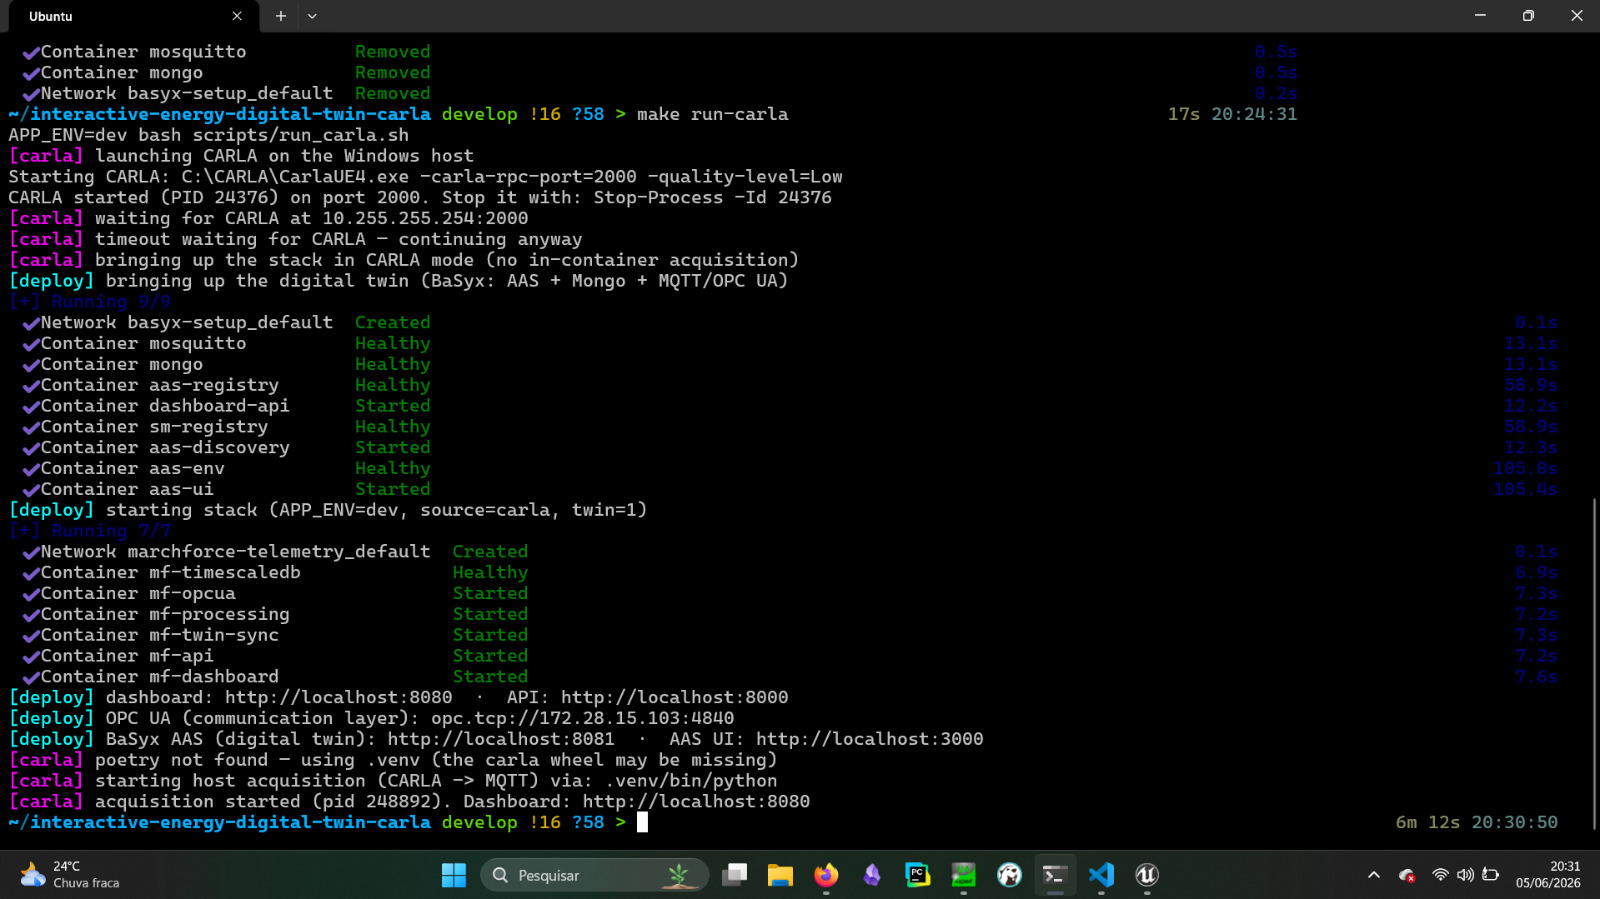
\includegraphics[width=\linewidth]{img/deploy_terminal.jpg}
\caption{Implantação por um comando: o CARLA, o gêmeo digital BaSyx (9 contêineres) e o \textit{stack} de telemetria (7 contêineres) sobem saudáveis, com os \textit{endpoints} publicados no IP do host.}
\label{fig:deploy}
\end{figure}

A operação do protótipo é padronizada por alvos de \code{make} (Tabela~\ref{tab:make}), garantindo reprodutibilidade: o mesmo comando builda as imagens enxutas, executa os testes como \textit{gate} de \textit{build} e sobe o \textit{stack}.

\begin{table}[h]
\centering
\caption{Principais comandos de operação (\code{make}).}
\label{tab:make}
\renewcommand{\arraystretch}{1.25}
\begin{tabular}{@{}ll@{}}
\toprule
\textbf{Comando} & \textbf{Descrição} \\
\midrule
\texttt{make run}         & Builda as imagens (testes como \textit{gate}) e sobe o \textit{stack} \\
\texttt{make run-carla}  & Inicia CARLA + \textit{stack} + lança aquisição no Windows automaticamente \\
\texttt{make carla-down} & Para containers, encerra aquisição e mata \texttt{CarlaUE4.exe} \\
\texttt{make verify}     & \textit{Smoke test} do \textit{stack} no ar (API, OPC UA, twin-sync) \\
\texttt{make test}       & Suíte unitária (\textit{pytest}, padrão AAA) \\
\texttt{make smoke}      & Pipeline ponta a ponta offline (\textit{fakes}, sem infraestrutura) \\
\texttt{make dev}        & Desenvolvimento com \textit{hot reload} (inclui twin-sync e BaSyx) \\
\texttt{make down}       & Derruba o \textit{stack} e a infra de telemetria (\texttt{timescaledb}) \\
\texttt{make report}     & Compila este relatório em PDF \\
\bottomrule
\end{tabular}
\end{table}

\section{Evolução Implementada}

Desde a versão inicial do documento, as seguintes evoluções foram implementadas:

\subsection*{Sistema de Logging Estruturado}
Foi implementado um sistema centralizado de logging utilizando a biblioteca \code{structlog}, configurado em \code{src/infra/logger.py}. A camada de domínio permanece livre de dependências de logging, conforme RNF1.

\subsection*{Barramento MQTT e Separação Aquisição/Processamento}
A aquisição (CARLA) publica leituras brutas no tópico \code{marchforce/telemetry/raw}. O serviço de processamento (\code{src/application/processing_service.py}) consome esse tópico, executa o modelo energético, persiste a série temporal e republica o estado processado em \code{marchforce/telemetry/processed}. O cliente MQTT~\cite{oasis_mqtt} (\code{src/infra/mqtt_client.py}) é o barramento lógico que desacopla os serviços; produtores e consumidores nunca se comunicam diretamente.

\subsection*{Persistência Temporal (TimescaleDB)}
O repositório \code{src/infra/timescale_repository.py} armazena a telemetria processada em PostgreSQL/TimescaleDB (hypertable), organizada por sessão de teste, permitindo consulta de histórico e comparação entre execuções via API REST.

\subsection*{Exposição via API REST + WebSocket e Dashboard Web}
A camada de exposição (\code{src/api/server.py}, FastAPI) entrega o histórico por REST e retransmite a telemetria processada por WebSocket. A dashboard (React + Vite) apresenta KPIs, gráficos em tempo real, painel de alertas, a pista do trajeto (coordenadas reais do CARLA) e modais de edição de parâmetros e limiares de alerta. Substitui a visualização HUD anterior.

\begin{figure}[h]
\centering
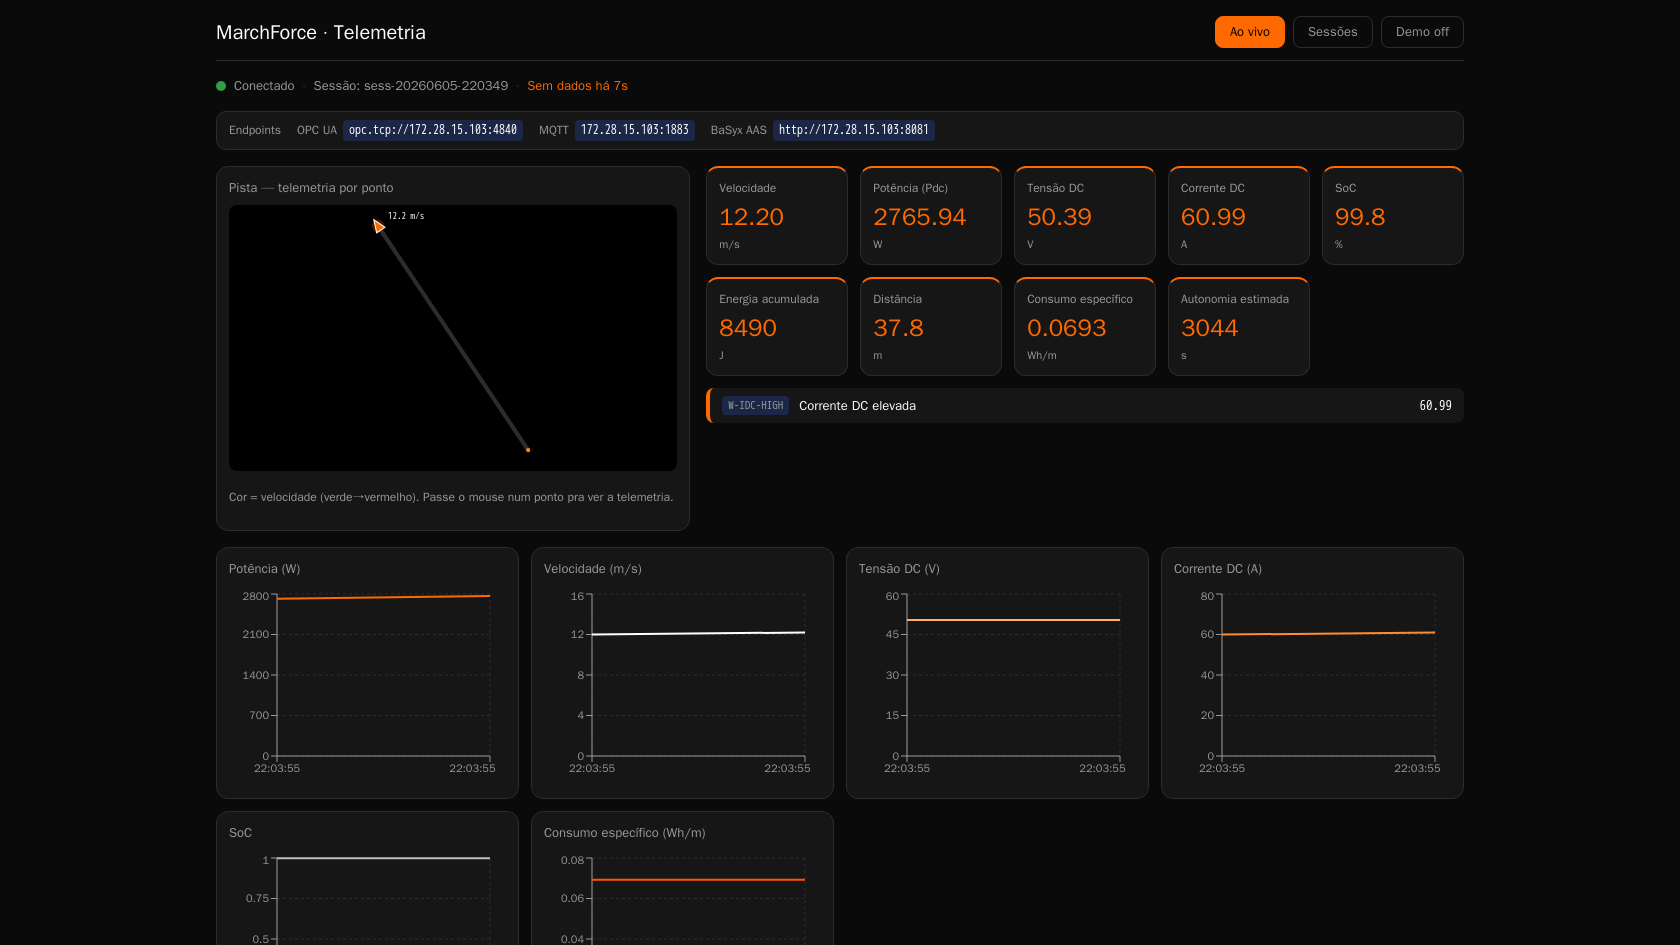
\includegraphics[width=\linewidth]{img/dashboard.png}
\caption{Dashboard web em tempo real (React + Vite): \textit{endpoints} no IP real do host, pista do trajeto, cartões de KPI, gráficos ao vivo e painel de alertas (no exemplo, o alerta \code{W-IDC-HIGH} de corrente DC elevada).}
\label{fig:dashboard}
\end{figure}

\subsection*{Conversões de Unidades na Dashboard}

O \textit{backend} e o barramento MQTT operam sempre em unidades SI (velocidade em m/s, energia em J, distância em m, consumo específico em Wh/m, autonomia em s). A conversão para unidades de usuário é feita exclusivamente na camada de apresentação (\code{KpiCards.jsx} e \code{LiveCharts.jsx}):

\begin{itemize}
  \item Velocidade: $\times 3{,}6 \Rightarrow$ km/h
  \item Energia acumulada: $\div 3600 \Rightarrow$ Wh
  \item Distância: $\times 0{,}001 \Rightarrow$ km
  \item Consumo específico: $\times 1000 \Rightarrow$ Wh/km
  \item Autonomia: convertida de segundos para o formato h\,min (ex.: \texttt{1h 23min} ou \texttt{47min})
\end{itemize}

A autonomia é tratada por uma função dedicada \code{fmtAutonomy(secs)}: retorna \texttt{—} para valores nulos, \texttt{0min} para zero, e usa o piso mínimo de 5\,W na potência média para evitar que o denominador seja zero (veículo parado, SoC calculado sobre potência negligível).

\subsection*{Integração com Asset Administration Shell (BaSyx)}
A classe \code{TwinService} (camada de Informação) realiza a sincronização com a AAS \code{vehicle-digitaltwin.aasx} via Eclipse BaSyx v2 (\textit{aas-environment}, API REST). Consumindo o tópico \code{marchforce/telemetry/processed}, o serviço atualiza em tempo real os KPIs do submodelo \textbf{EnergyEfficiency} (\code{Distance}, \code{AveragePower}, \code{SpecificConsumption} e \code{Autonomy}) por PATCH REST, de forma \emph{orientada ao modelo canônico} (\code{aas_model.TELEMETRY_MODEL}). A série temporal crua não é replicada na AAS: ela é referenciada pelo \code{LinkedSegment} do submodelo \code{TimeSeries} (apontando para o TimescaleDB via API), conforme o SMT IDTA 02008. Assim, mantém-se uma única fonte de dados (sem segunda execução do CARLA) e a AAS permanece uma representação dinâmica do ativo.

\begin{figure}[h]
\centering
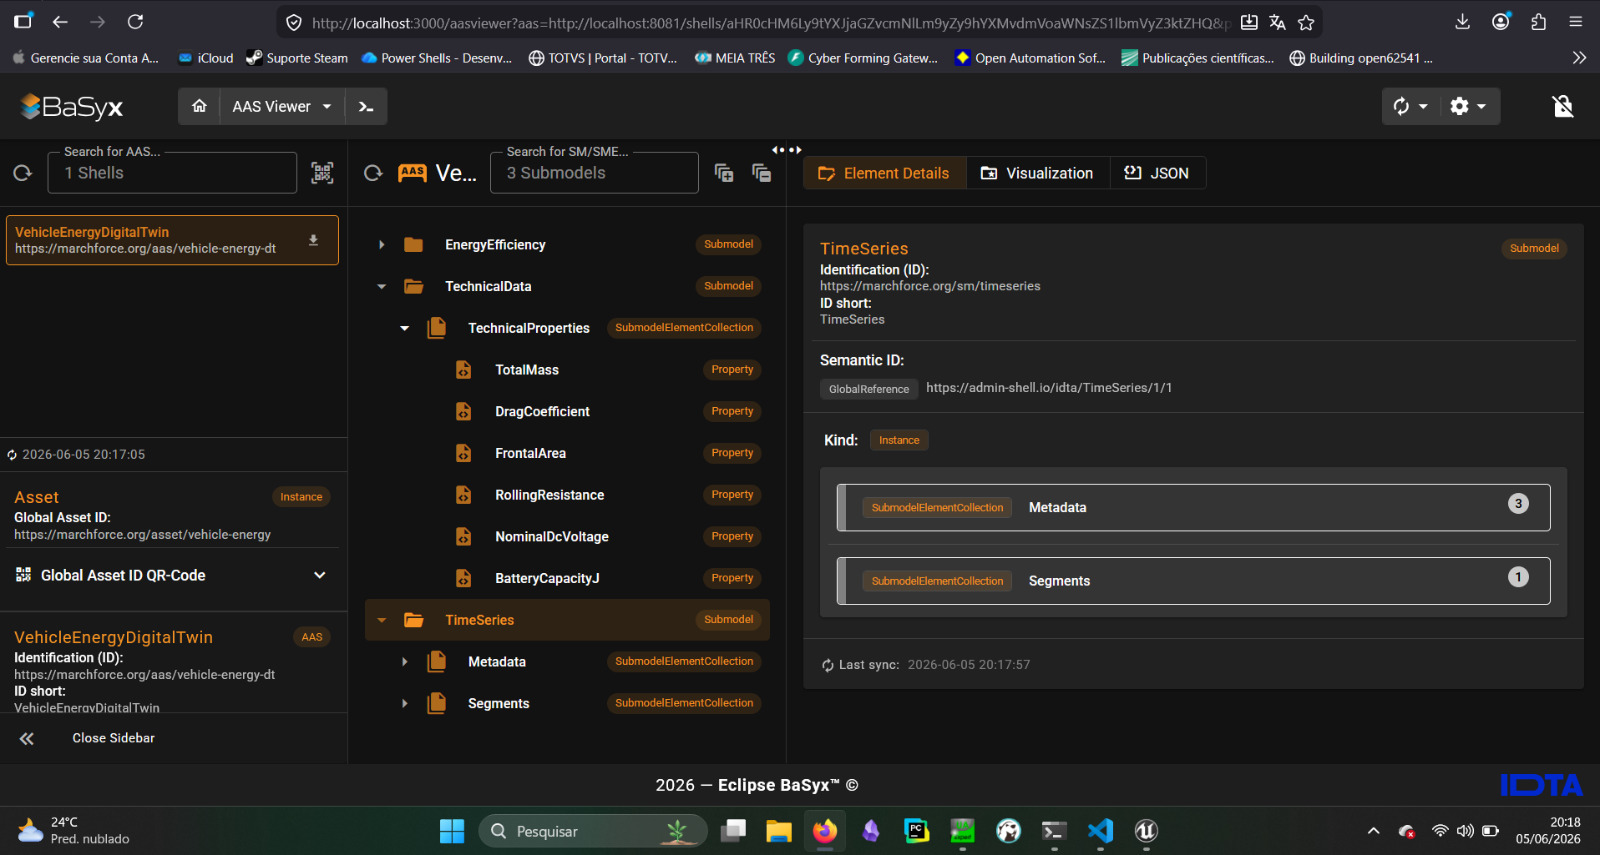
\includegraphics[width=\linewidth]{img/basyx_ui.jpg}
\caption{Asset Administration Shell carregada no Eclipse BaSyx Web UI: a \textit{shell} \code{VehicleEnergyDigitalTwin} e os três submodelos IDTA (\code{EnergyEfficiency}, \code{TechnicalData} e \code{TimeSeries}).}
\label{fig:basyx}
\end{figure}

A AAS efetivamente carregada e sincronizada foi verificada pela API REST do
BaSyx (Listagem~\ref{lst:basyx}): a \textit{shell} e os três submodelos IDTA
aparecem, e o submodelo \code{EnergyEfficiency} exibe os KPIs já atualizados
pelo \textit{twin-sync}.

\begin{figure}[h]
\centering
\begin{evidencia}
\begin{Verbatim}[fontsize=\small]
GET /shells     -> ["VehicleEnergyDigitalTwin"]
GET /submodels  -> ["TimeSeries", "EnergyEfficiency", "TechnicalData"]
GET /submodels/<EnergyEfficiency>/submodel-elements
   Distance            = 358.5
   AveragePower        = 1665.45
   SpecificConsumption = 0.0494
   Autonomy            = 2963.9
\end{Verbatim}
\end{evidencia}
\caption{Evidência REST: AAS carregada no BaSyx v2 e KPIs de \code{EnergyEfficiency} atualizados pelo \textit{twin-sync}.}
\label{lst:basyx}
\end{figure}

A AAS também pode ser inspecionada pelo BaSyx Web UI (Figura~\ref{fig:basyx}) e pela API REST documentada em \textit{Swagger} (Figura~\ref{fig:swagger}).

\begin{figure}[h]
\centering
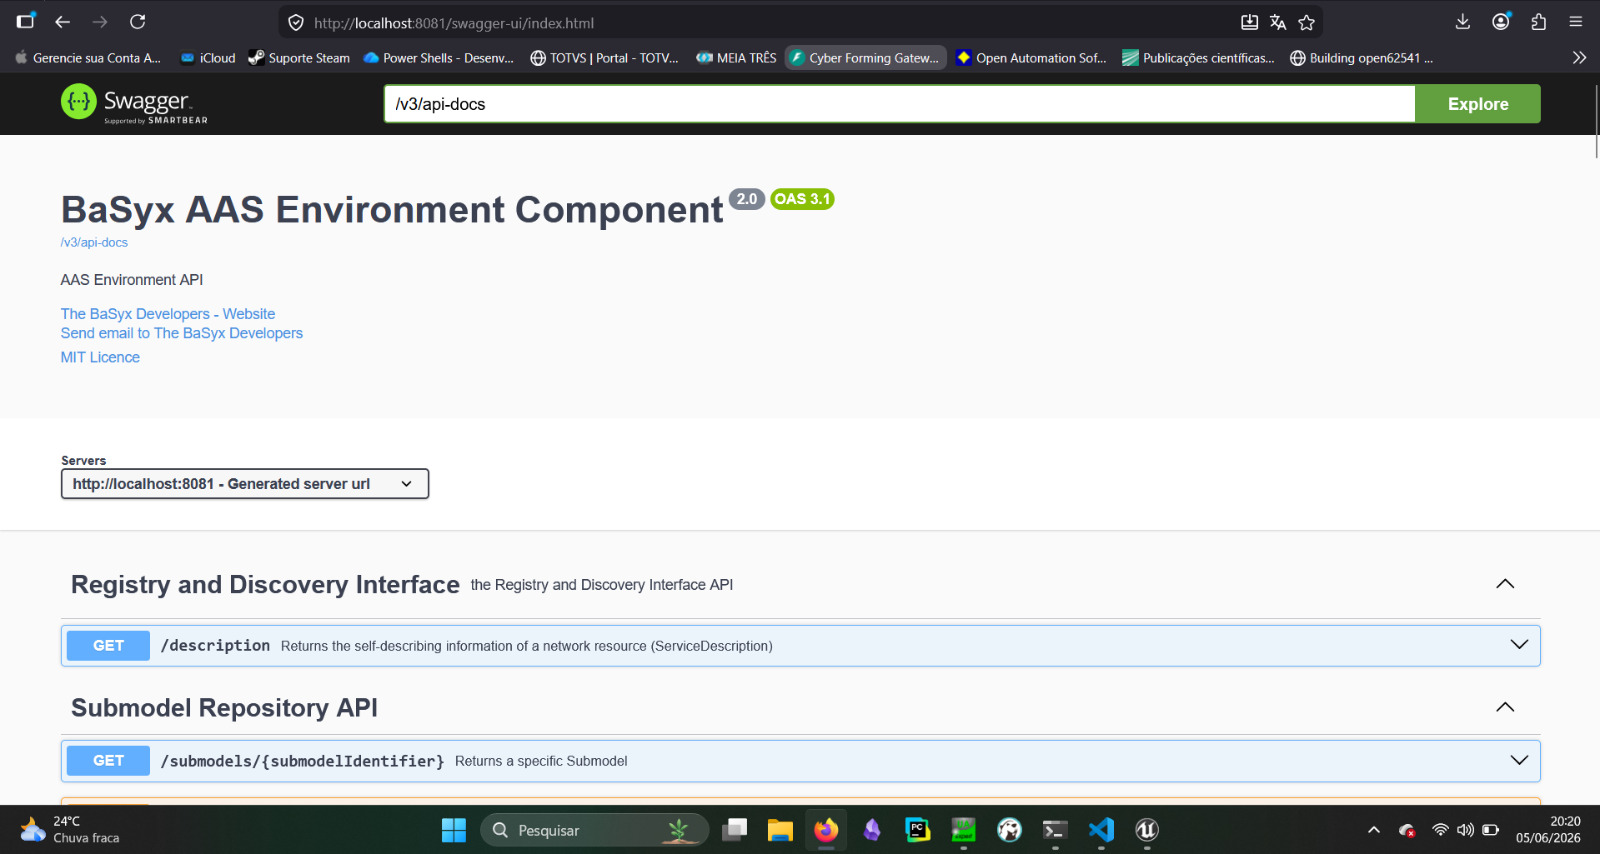
\includegraphics[width=\linewidth]{img/basyx_swagger.jpg}
\caption{API REST do BaSyx v2 (\textit{aas-environment}, OpenAPI 3.1) usada pelo \textit{twin-sync} para sincronizar os submodelos.}
\label{fig:swagger}
\end{figure}

\subsection*{Exposição AAS via MQTT}

Além da sincronização REST com o BaSyx, o \code{TwinSyncService} publica cada elemento dos submodelos AAS como tópico MQTT independente, imediatamente após cada ciclo de PATCH. A estrutura de tópicos segue a hierarquia \code{marchforce/aas/\{Submodelo\}/\{idShort\}}, por exemplo:

\begin{itemize}
  \item \code{marchforce/aas/TimeSeries/Velocity} --- velocidade em m/s
  \item \code{marchforce/aas/TimeSeries/InstantaneousPower} --- potência em W
  \item \code{marchforce/aas/EnergyEfficiency/Distance} --- distância em m
  \item \code{marchforce/aas/EnergyEfficiency/Autonomy} --- autonomia em s
\end{itemize}

Isso torna a estrutura da AAS diretamente observável por qualquer cliente MQTT (e.g., MQTT Explorer), sem necessidade de acesso à API REST do BaSyx. A publicação usa os mesmos valores e escalas definidos no modelo canônico (\code{aas_model.TELEMETRY_MODEL}), garantindo coerência entre REST, OPC UA e MQTT. A assinatura curinga \code{marchforce/aas/\#} entrega todos os elementos de ambos os submodelos dinâmicos.

\subsection*{Integração OPC UA (RF8: Camada de Comunicação)}
Foi implementado o servidor OPC UA em \code{src/application/opcua_service.py} com a biblioteca \code{asyncua}. O servidor é \emph{totalmente parametrizado por ambiente} (host, porta, \textit{path}, \textit{namespace}, nome do servidor e intervalo de atualização), sem valores fixos no código (RNF5). Ele consome o tópico \code{marchforce/telemetry/processed} e expõe a \textit{shell} do gêmeo digital, cujos nós são atualizados periodicamente.

Um ponto central de projeto é que a \emph{estrutura de nós OPC UA é construída a partir do modelo canônico} (\code{src/domain/aas_model.py}, \code{TELEMETRY_MODEL}), o mesmo que origina o \code{Record} da AAS, \textbf{espelhando a hierarquia do AAS V3}: o objeto raiz recebe o \textit{idShort} da \textit{shell} (\code{VehicleEnergyDigitalTwin}) e dela pendem, como filhos diretos, os três submodelos. Assim, em vez de uma lista plana de variáveis, os nós ficam \emph{agrupados por submodelo}: \code{TimeSeries} (com \code{Velocity}, \code{Acceleration}, \code{InstantaneousPower}, \code{AccumulatedEnergy}, \code{DcVoltage}, \code{DcCurrent}, \code{StateOfCharge}), \code{EnergyEfficiency} (com \code{Distance}, \code{AveragePower}, \code{SpecificConsumption}, \code{Autonomy}) e \code{TechnicalData} (parâmetros estáticos do veículo). Os \code{idShort} OPC UA coincidem com os da AAS, garantindo uma única fonte estrutural: alterar o modelo canônico reflete simultaneamente na AAS e no espaço de endereçamento OPC UA. Endpoint padrão: \code{opc.tcp://<host>:4840/marchforce/}, conectável por clientes como o UAExpert.

Cabe registrar a fronteira RAMI~4.0 adotada: o servidor \code{asyncua} provê a \emph{camada de Comunicação} (protocolo OPC UA~\cite{iec62541}), enquanto o BaSyx serve a AAS pela API REST (camada de Informação). \textbf{Hoje, OPC UA e AAS são alimentados em paralelo pelo mesmo barramento MQTT} (exposição paralela); não há, ainda, uma ponte canônica OPC~UA~$\rightarrow$~AAS. Essa integração, via BaSyx \textit{DataBridge}, é trabalho futuro.

\begin{figure}[h]
\centering
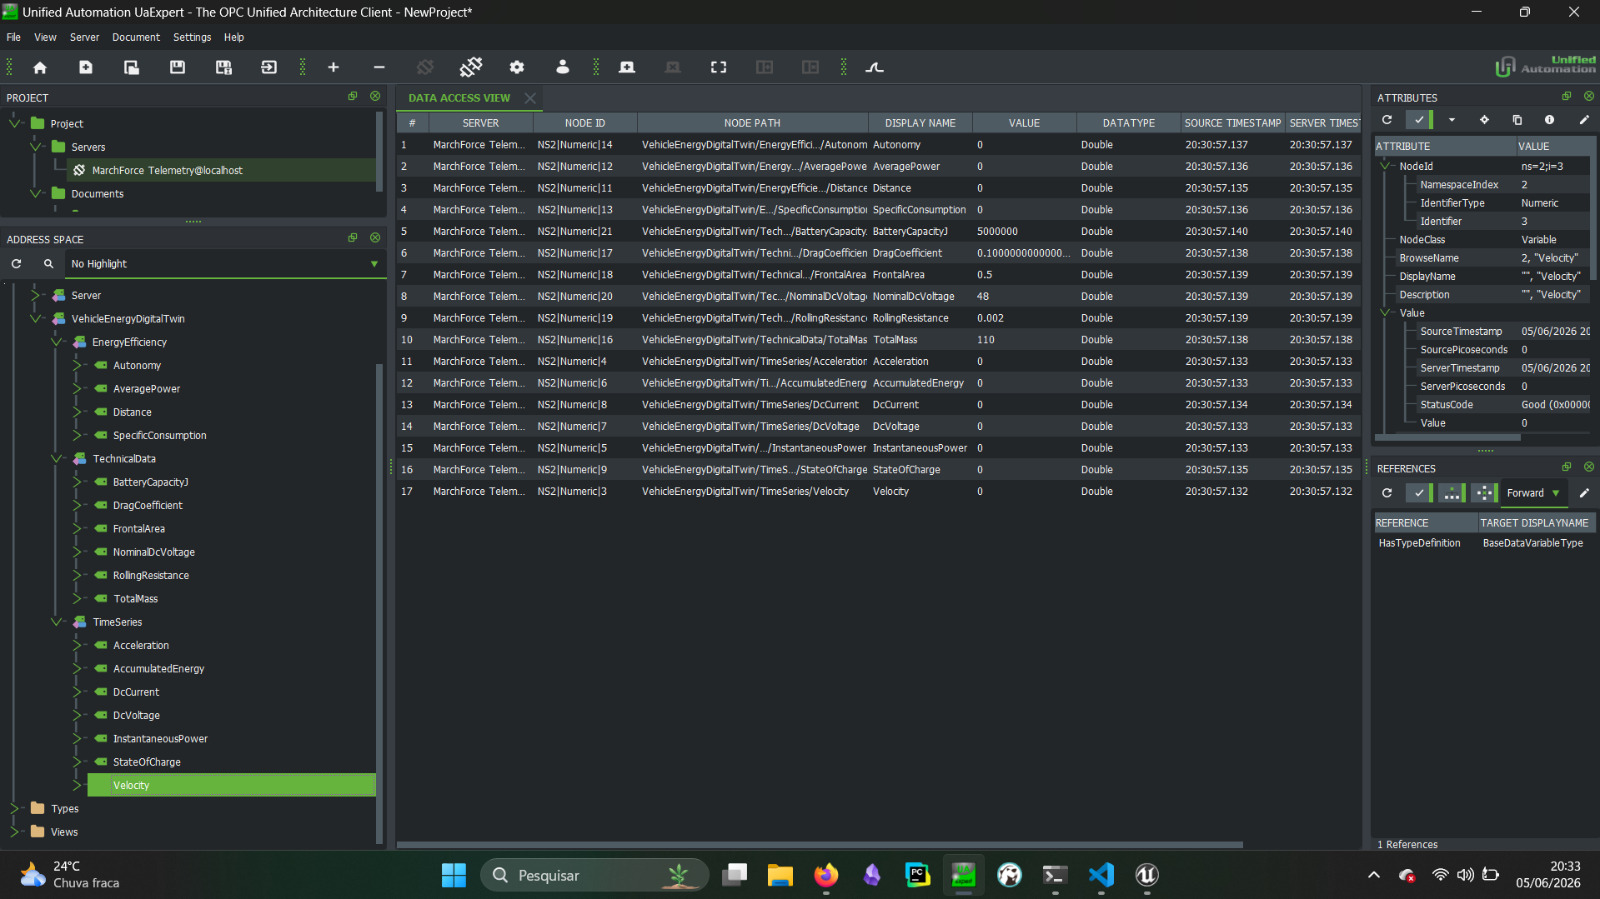
\includegraphics[width=\linewidth]{img/uaexpert.jpg}
\caption{Servidor OPC UA inspecionado no UAExpert: a \textit{shell} \code{VehicleEnergyDigitalTwin} como raiz, os submodelos \code{EnergyEfficiency}, \code{TechnicalData} e \code{TimeSeries} como filhos diretos, e os valores atualizando em tempo real.}
\label{fig:opcua}
\end{figure}

O espaço de endereçamento foi inspecionado por um cliente OPC UA
(Listagem~\ref{lst:opcua}), confirmando os nós agrupados por submodelo e os
valores atualizando a partir do barramento MQTT.

\begin{figure}[h]
\centering
\begin{evidencia}
\begin{Verbatim}[fontsize=\small]
opc.tcp://172.28.15.103:4840/marchforce/
`-- VehicleEnergyDigitalTwin        (shell / AAS)
    |-- TimeSeries
    |   |-- Velocity            = 30.00
    |   |-- Acceleration        = 0.00
    |   |-- InstantaneousPower  = 891.62
    |   |-- AccumulatedEnergy   = 69047.53
    |   |-- DcVoltage           = 50.33
    |   |-- DcCurrent           = 19.69
    |   `-- StateOfCharge       = 98.47
    |-- EnergyEfficiency
    |   |-- Distance            = 891.88
    |   |-- AveragePower        = 891.62
    |   |-- SpecificConsumption = 0.023894
    |   `-- Autonomy            = 5521.7
    `-- TechnicalData
        |-- TotalMass           = 110.0
        |-- DragCoefficient     = 0.10
        |-- FrontalArea         = 0.5
        |-- RollingResistance   = 0.002
        |-- NominalDcVoltage    = 48.0
        `-- BatteryCapacityJ    = 5000000.0
\end{Verbatim}
\end{evidencia}
\caption{Árvore de nós OPC UA lida por cliente (\code{asyncua}): a \textit{shell} \code{VehicleEnergyDigitalTwin} como raiz e os submodelos \code{TimeSeries}, \code{EnergyEfficiency} e \code{TechnicalData} como filhos diretos (AAS V3).}
\label{lst:opcua}
\end{figure}

O servidor é localizável na rede tanto em \code{localhost} quanto no IP real do host (Figura~\ref{fig:opcua_disc}), de modo que clientes externos (e.g., o \textit{box} ou uma ferramenta de engenharia) o descobrem e conectam, aqui com autenticação anônima.

\begin{figure}[h]
\centering
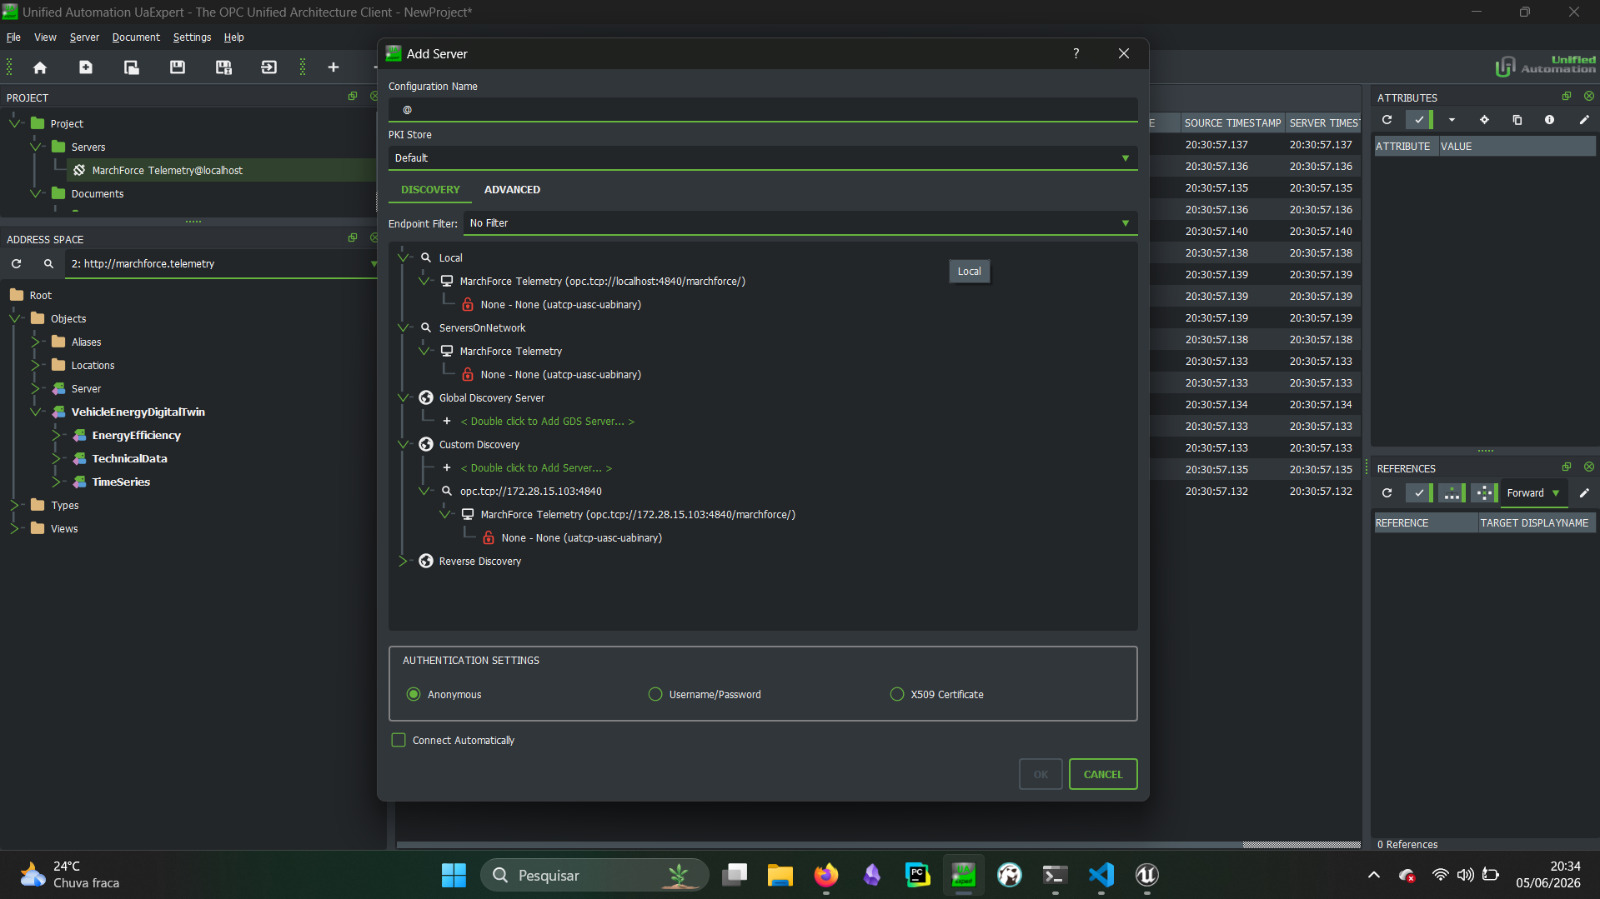
\includegraphics[width=\linewidth]{img/uaexpert_discovery.jpg}
\caption{Descoberta do servidor OPC UA no UAExpert: o \textit{endpoint} \texttt{MarchForce Telemetry} é encontrado em \code{opc.tcp://localhost:4840/marchforce/} e no IP real do host (\code{opc.tcp://172.28.15.103:4840/marchforce/}).}
\label{fig:opcua_disc}
\end{figure}

\subsection*{Enlace LoRa (Telemetria Externa)}
O serviço \code{src/application/lora_service.py} consome o barramento processado e transmite um subconjunto de variáveis essenciais e alertas críticos ao box, respeitando MTU pequeno e duty cycle. O enlace é um \textit{port} \code{TelemetryLink}, com adaptadores de \textit{log} (sem hardware) e serial.

\subsection*{Diagnóstico e Alertas Operacionais}
O módulo \code{src/domain/diagnostics.py} avalia cada amostra e emite alertas com código (\code{AlertCode}), severidade (\code{Severity}) e mensagem, propagados no barramento e exibidos na dashboard, cobrindo SoC, tensão/corrente DC, velocidade, leituras inválidas e falhas de persistência.

\section{Estrutura de Submodelos AAS (conforme IDTA)}

A modelagem da Asset Administration Shell~\cite{plattform_aas} segue os \textit{Submodel Templates} (SMTs) padronizados da \textit{Industrial Digital Twin Association} (IDTA)~\cite{idta02008}, garantindo interoperabilidade. A AAS (\code{aas-model/vehicle-digitaltwin.aasx}) é composta por três submodelos (Tabela~\ref{tab:aas}):

\begin{itemize}
    \item \textbf{TimeSeries} (IDTA 02008-1-1 \textit{Time Series Data}, \code{semanticId} \code{https://admin-shell.io/idta/TimeSeries/1/1}): descreve a telemetria \emph{dinâmica}. O \code{Metadata/Record} define o \textit{schema} das variáveis e o \code{Segments/LinkedSegment} referencia a base temporal (TimescaleDB) via \code{Endpoint}/\code{Query} da API, sem duplicar os dados na AAS.
    \item \textbf{EnergyEfficiency}: KPIs \emph{derivados} de gestão de energia, atualizados em tempo real na AAS via PATCH REST.
    \item \textbf{TechnicalData} (IDTA 02003): parâmetros \emph{estáticos} do veículo.
\end{itemize}

\begin{table}[h]
\centering
\caption{Submodelos AAS (IDTA) e variáveis}
\label{tab:aas}
\begin{tabular}{@{}llll@{}}
\toprule
\textbf{Submodelo (SMT)} & \textbf{Elemento (idShort)} & \textbf{Variável} & \textbf{Natureza} \\
\midrule
TimeSeries (02008)       & Record.Velocity             & $v_{long}$   & dinâmica (DB)  \\
TimeSeries (02008)       & Record.Acceleration         & $a_{long}$   & dinâmica (DB)  \\
TimeSeries (02008)       & Record.InstantaneousPower   & $P$          & dinâmica (DB)  \\
TimeSeries (02008)       & Record.AccumulatedEnergy    & $E$          & dinâmica (DB)  \\
TimeSeries (02008)       & Record.DcVoltage            & $V_{dc}$     & dinâmica (DB)  \\
TimeSeries (02008)       & Record.DcCurrent            & $I_{dc}$     & dinâmica (DB)  \\
TimeSeries (02008)       & Record.StateOfCharge        & $SoC$        & dinâmica (DB)  \\
\midrule
EnergyEfficiency         & Distance                    & $d$          & dinâmica (PATCH) \\
EnergyEfficiency         & AveragePower                & $\bar{P}$    & dinâmica (PATCH) \\
EnergyEfficiency         & SpecificConsumption         & $C_{esp}$    & dinâmica (PATCH) \\
EnergyEfficiency         & Autonomy                    & $A$          & dinâmica (PATCH) \\
\midrule
TechnicalData (02003)    & TotalMass                   & $m$          & estática \\
TechnicalData (02003)    & DragCoefficient             & $C_d$        & estática \\
TechnicalData (02003)    & FrontalArea                 & $A_f$        & estática \\
TechnicalData (02003)    & RollingResistance           & $C_r$        & estática \\
TechnicalData (02003)    & NominalDcVoltage            & $V_{nom}$    & estática \\
TechnicalData (02003)    & BatteryCapacityJ            & $C_{bat}$    & estática \\
\bottomrule
\end{tabular}
\end{table}

A série temporal crua é exposta pelo \code{LinkedSegment} (apontando para o TimescaleDB via API), enquanto os KPIs de eficiência são atualizados na AAS via PATCH REST do BaSyx v2 (\code{/submodels/{base64(submodelId)}/submodel-elements/{idShort}/$value}), alimentados pelo consumo do tópico \code{marchforce/telemetry/processed}. Os identificadores seguem codificação Base64 URL-safe conforme AAS Part 2. O arquivo \code{.aasx} foi validado com o \code{basyx-python-sdk}.

\subsection*{Indicadores Estratégicos de Eficiência}

A classe \code{VehicleEnergySystem} calcula:
\begin{itemize}
    \item \textbf{Distância acumulada}:
          \begin{equation} d(t) = \sum_{k=0}^{n} |v_k| \cdot \Delta t \end{equation}
    \item \textbf{Potência média móvel} (janela de 50 passos):
          \begin{equation} \bar{P}(t) = \frac{1}{N} \sum_{i=t-N}^{t} P(i) \end{equation}
    \item \textbf{Consumo específico}:
          \begin{equation} C_{esp} = \frac{E_{elec} / 3600}{d} \quad [\text{Wh/m}] \end{equation}
    \item \textbf{Autonomia estimada}:
          \begin{equation} A(t) = \frac{SoC \cdot C_{bat}}{\bar{P}(t)} \quad [\text{s}] \end{equation}
          A estimativa é definida apenas quando $\bar{P}(t)$ supera um piso mínimo, evitando divisão por valores próximos de zero (carro parado/cruzeiro).
\end{itemize}

\subsection*{Validação por Testes Unitários}

Foram implementados 89 testes unitários, no padrão Arrange--Act--Assert, cobrindo:
\begin{itemize}
    \item \code{EnergyModel}: cálculo de forças, potência, acumulação de energia
    \item \code{Battery}: descarga, regeneração, limitação do SoC
    \item \code{VehicleEnergySystem}: indicadores estratégicos, distância, média móvel
    \item \code{Diagnostics}: enums, limiares e geração de alertas
    \item Serviços (aquisição, processamento, LoRa, twin-sync) com \textit{fakes} que implementam as portas, sem broker ou banco
    \item Configuração, fontes, portas e hierarquia de exceções
\end{itemize}

A validação offline confirma RNF2.

\subsection*{Simulação Sintética}

O script \code{scripts/simulate.py} executa o pipeline energético completo sem dependência de CARLA/BaSyx, com três fases: aceleração (0--15\,s), cruzeiro (15--40\,s) e frenagem regenerativa (40--60\,s). Um \textit{smoke test} (\code{scripts/smoke_pipeline.py}) valida o caminho ponta a ponta (fonte $\rightarrow$ processamento $\rightarrow$ consumidores) sem infraestrutura externa.

\section{Aquisição de Variáveis do CARLA}

O simulador fornece velocidade como vetor 3D. Para a componente longitudinal, projeta-se no \textit{forward vector}:

\begin{equation}
    v_{long} = \vec{v} \cdot \hat{f} = v_x f_x + v_y f_y + v_z f_z
\end{equation}

Onde $\hat{f}$ é obtido via \code{vehicle.get_transform().get_forward_vector()}.

A aceleração longitudinal é derivada da velocidade entre passos consecutivos, filtrada por média móvel exponencial e limitada a uma faixa física, evitando picos não-físicos da leitura bruta do simulador (colisões/ruído):

\begin{equation}
    a_{long}(t) = \mathrm{clamp}\!\left( \frac{v_{long}(t) - v_{long}(t-\Delta t)}{\Delta t},\; -a_{max},\; a_{max} \right)
\end{equation}

O veículo é conduzido no simulador por teclado (WASD, com \code{S} acionando a ré) e acompanhado por uma câmera de perseguição. A aquisição roda no host Windows (única plataforma suportada pela \textit{wheel} \code{win\_amd64} do CARLA) e publica as leituras no barramento MQTT; o script \code{run\_carla.sh} a lança automaticamente via \code{powershell.exe}, eliminando a necessidade de abrir um terminal separado.

O \textit{spawn} do veículo utiliza \code{try\_spawn\_actor()} em um laço que itera todos os pontos de \textit{spawn} disponíveis no mapa, evitando falha quando o ponto padrão está ocupado por sessões anteriores não encerradas. A aquisição roda no host e publica as leituras no barramento MQTT, de modo que a dashboard desenha o trajeto e exibe a telemetria energética em tempo real, sem nenhum acoplamento entre o domínio e o simulador (Figuras~\ref{fig:carla} e~\ref{fig:carla_car}).

\begin{figure}[h]
\centering
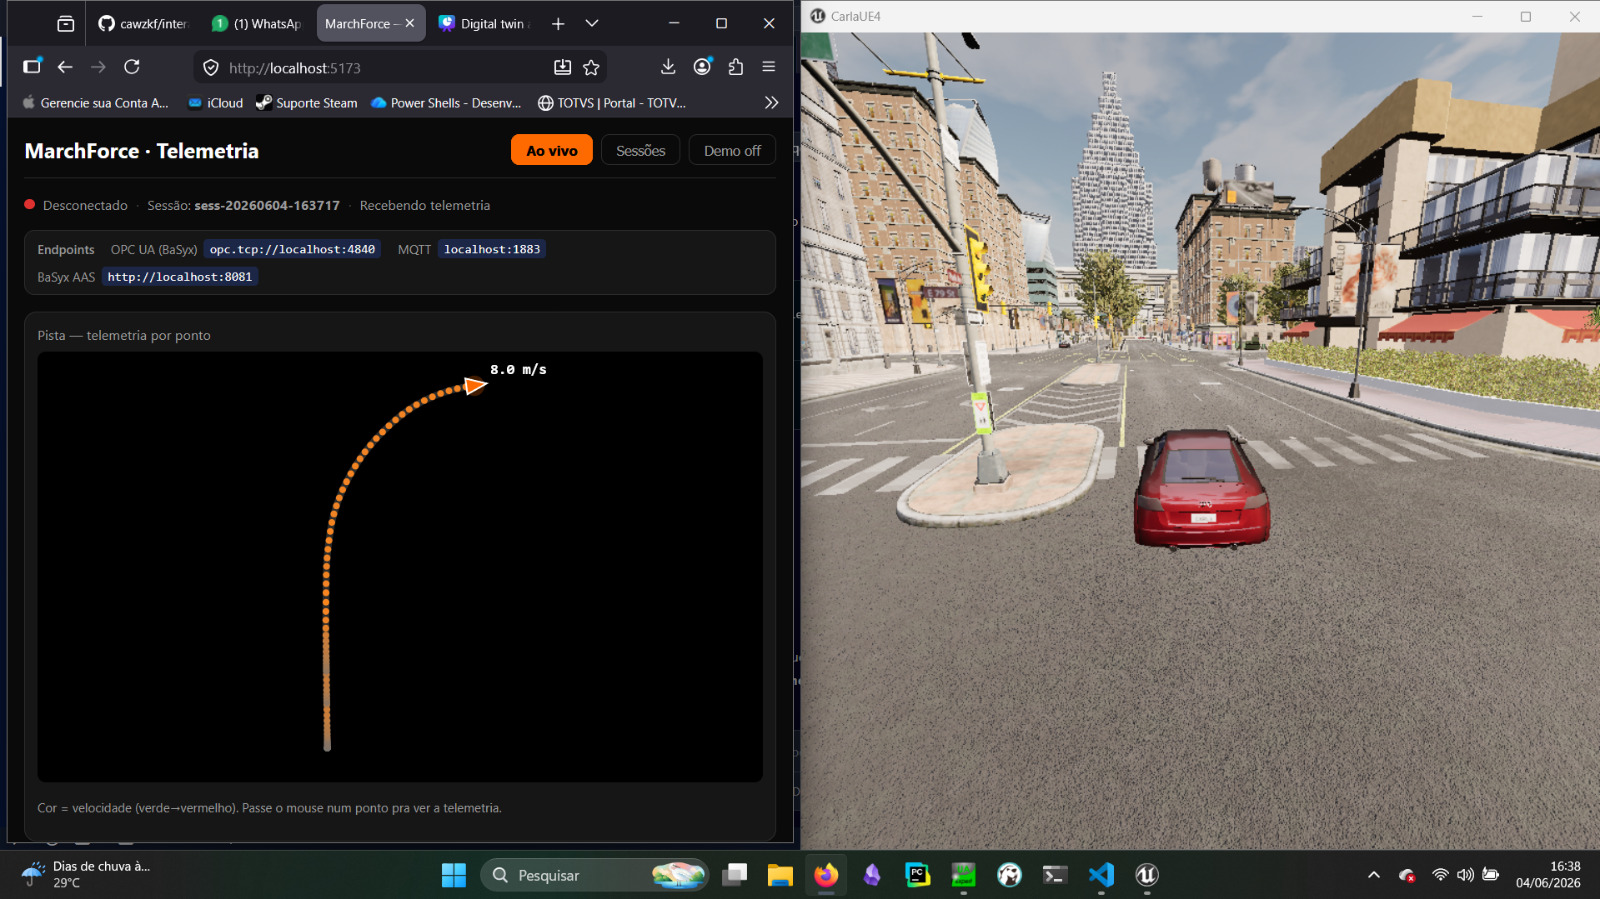
\includegraphics[width=\linewidth]{img/carla_split.jpg}
\caption{Aquisição com CARLA: à direita o veículo é dirigido no simulador (WASD, câmera de perseguição); à esquerda a dashboard recebe a telemetria pelo barramento e desenha o trajeto em tempo real.}
\label{fig:carla}
\end{figure}

\begin{figure}[h]
\centering
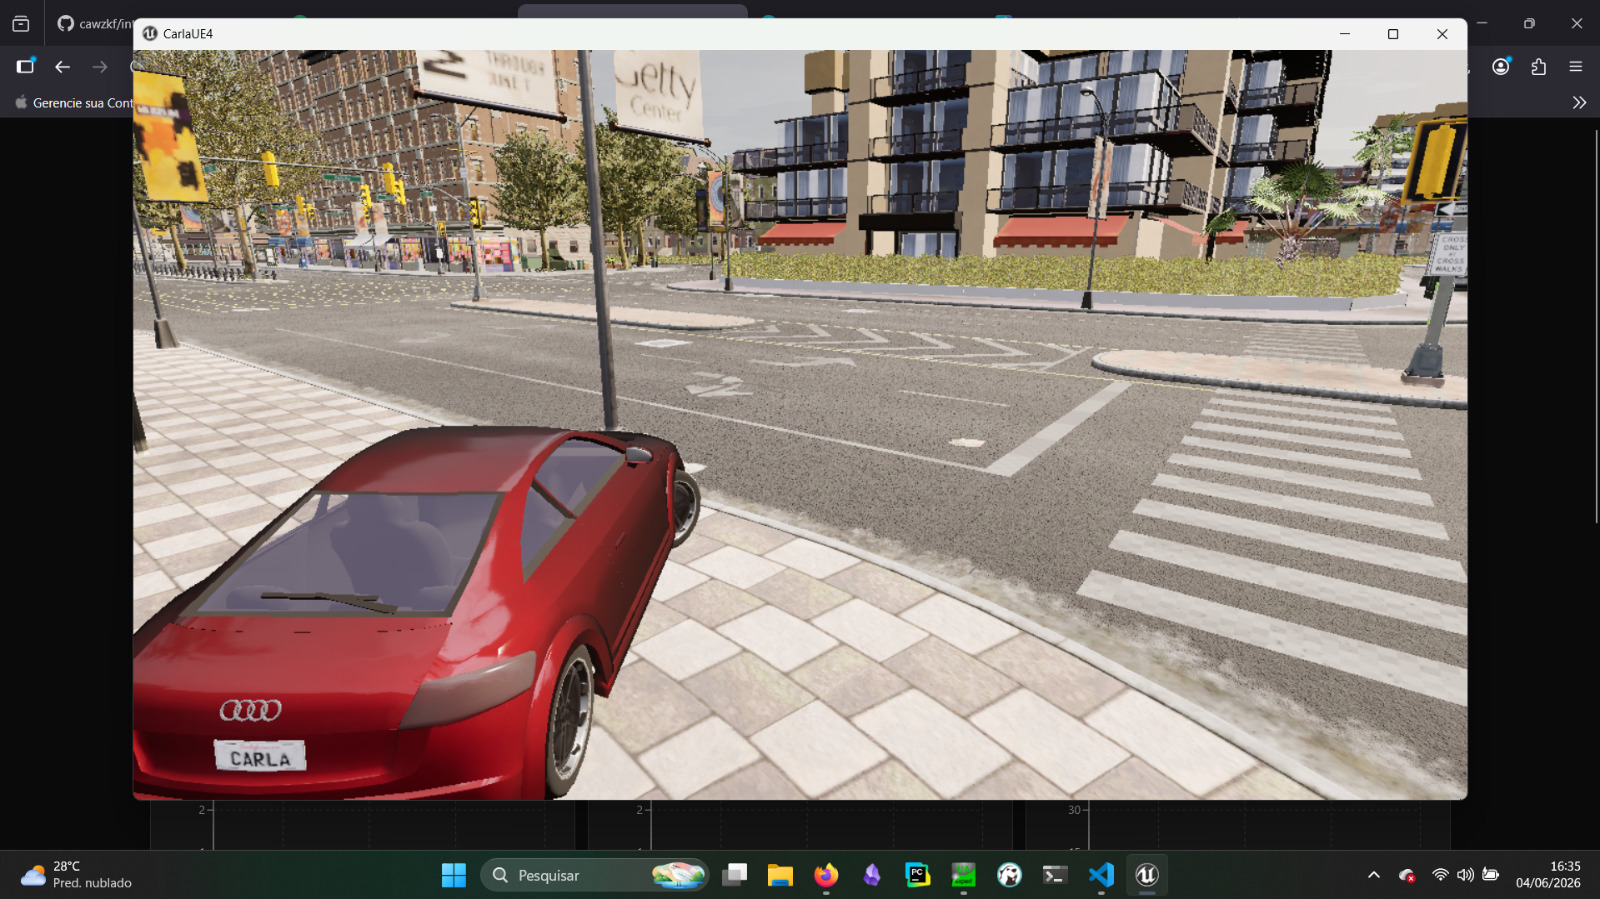
\includegraphics[width=0.7\linewidth]{img/carla_car.jpg}
\caption{Veículo no CARLA com câmera de perseguição, controlado por teclado (WASD; \code{S} aciona a ré).}
\label{fig:carla_car}
\end{figure}

\chapter{Fundamentação Teórica}

\section{Digital Twin}

O conceito de \textit{Digital Twin} foi formalizado por Grieves \cite{grieves2014digital}, sendo expandido como integração dinâmica entre sistemas físicos e modelos computacionais conectados em tempo real \cite{fuller2020digital}.

Neste trabalho considera-se apenas dinâmica longitudinal em plano horizontal.

\section{RAMI 4.0}

O \textit{Reference Architectural Model Industrie 4.0} (RAMI 4.0)~\cite{din91345} organiza sistemas ciberfísicos em camadas hierárquicas: Ativo, Integração, Comunicação, Informação, Funcional e Negócio. Este trabalho atende explicitamente as cinco primeiras (Figura~\ref{fig:rami}): o OPC UA é o protocolo da camada de Comunicação (servidor \code{asyncua}), e o MQTT, a persistência temporal e o AAS/BaSyx compõem a camada de Informação. Cabe destacar que, no Eclipse BaSyx v2, o \textit{aas-environment} expõe o AAS por REST; a integração canônica de protocolos de campo (OPC UA, MQTT) ao AAS é feita pelo componente \textit{DataBridge} (cliente), prevista como evolução.

\begin{figure}[h]
\centering
\begin{tikzpicture}[font=\sffamily,
  layer/.style={minimum width=5cm, minimum height=0.92cm, align=center, font=\sffamily\bfseries\small, text=white},
  cov/.style={layer, fill=mfSteel}, hot/.style={layer, fill=mfOrange},
  off/.style={layer, fill=mfRule, text=mfGraphite},
  map/.style={anchor=west, font=\sffamily\small, text=mfInk}]
  \node[off] (l6) at (0,0)    {Negócio};
  \node[cov] (l5) at (0,-1.0) {Funcional};
  \node[cov] (l4) at (0,-2.0) {Informação};
  \node[cov] (l3) at (0,-3.0) {Comunicação};
  \node[cov] (l2) at (0,-4.0) {Integração};
  \node[hot] (l1) at (0,-5.0) {Ativo};
  \draw[mfOrange, line width=3pt] (-2.62,-5.46) -- (-2.62,-0.54);
  \node[map] at (2.85,0)    {\itshape fora do escopo deste protótipo};
  \node[map] at (2.85,-1.0) {Modelo energético, diagnóstico e processamento};
  \node[map] at (2.85,-2.0) {MQTT, TimescaleDB e AAS via BaSyx};
  \node[map] at (2.85,-3.0) {Servidor OPC UA, API/WebSocket e LoRa};
  \node[map] at (2.85,-4.0) {Aquisição do CARLA (RS485/B.O.M. no futuro)};
  \node[map] at (2.85,-5.0) {Veículo (simulado no CARLA)};
\end{tikzpicture}
\caption{Camadas da RAMI 4.0 e o mapeamento para os componentes do protótipo. As cinco camadas inferiores (Ativo a Funcional) são atendidas; a camada de Negócio está fora do escopo.}
\label{fig:rami}
\end{figure}

\section{Modelo Longitudinal Simplificado}

Modelos longitudinais são discutidos na literatura de dinâmica veicular \cite{rajamani2011vehicle}:

\begin{equation} F_{rol} = C_r \, m \, g \end{equation}
\begin{equation} F_{aero} = \frac{1}{2} \rho C_d A v^2 \end{equation}
\begin{equation} F_{long} = m \cdot a + F_{rol} + F_{aero} \end{equation}

Onde $m$ é a massa [kg], $a$ a aceleração [m/s²], $C_r$ o coeficiente de rolamento, $g$ a gravidade [m/s²], $\rho$ a densidade do ar [kg/m³], $C_d$ o coeficiente aerodinâmico, $A$ a área frontal [m²] e $v$ a velocidade [m/s].

A modelagem de bateria segue abordagem energética de alto nível \cite{larminie2012electric}.

\begin{equation} P = F_{long} \cdot v \end{equation}
\begin{equation} E = \int P \, dt \end{equation}
\begin{equation} E_k = E_{k-1} + P_k \cdot \Delta t \end{equation}

\section{Convenção de Sinal e Regime Regenerativo}

\begin{itemize}
    \item $P > 0$: tração -- energia da bateria
    \item $P = 0$: equilíbrio
    \item $P < 0$: frenagem regenerativa -- energia à bateria
\end{itemize}

\begin{equation} E_{elec} = \frac{P \cdot \Delta t}{\eta_d} \end{equation}
\begin{equation} E_{regen} = |P| \cdot \Delta t \cdot \eta_r \end{equation}
\begin{equation} SoC_{k+1} = SoC_k - \frac{E_{elec}}{C_{bat}} \quad \text{(tração)} \end{equation}
\begin{equation} SoC_{k+1} = \min\left(1,\; SoC_k + \frac{E_{regen}}{C_{bat}}\right) \quad \text{(regeneração)} \end{equation}

\section{Parâmetros do Modelo}

Os parâmetros são configuráveis por ambiente (RNF5). A Tabela~\ref{tab:params} apresenta a configuração de referência utilizada na verificação analítica (veículo de passeio). O \textit{deploy} de produção adota uma configuração de protótipo leve (e.g., massa total $\approx$110\,kg, $C_d \approx 0{,}10$, $A \approx 0{,}5$\,m$^2$, $C_r \approx 0{,}002$), editável em tempo de execução pela dashboard.

\begin{table}[h]
\centering
\caption{Parâmetros de referência do modelo energético (verificação)}
\label{tab:params}
\begin{tabular}{@{}llll@{}}
\toprule
\textbf{Parâmetro} & \textbf{Símbolo} & \textbf{Valor} & \textbf{Unidade} \\
\midrule
Massa do veículo          & $m$     & 1500   & kg      \\
Coeficiente aerodinâmico  & $C_d$   & 0,3    & --      \\
Área frontal              & $A$     & 2,2    & m$^2$   \\
Coeficiente de rolamento  & $C_r$   & 0,015  & --      \\
Densidade do ar           & $\rho$  & 1,225  & kg/m$^3$\\
Aceleração da gravidade   & $g$     & 9,81   & m/s$^2$ \\
Capacidade da bateria     & $C_{bat}$ & 50   & MJ      \\
Eficiência de descarga    & $\eta_d$  & 0,9  & --      \\
Eficiência de regeneração & $\eta_r$  & 0,9  & --      \\
Passo de simulação        & $\Delta t$ & 0,1 & s       \\
\bottomrule
\end{tabular}
\end{table}

Os parâmetros do veículo e os limiares de alerta são, ainda, editáveis em tempo de execução pela dashboard (Figura~\ref{fig:modal}): o modal publica a nova configuração no tópico \code{marchforce/config}, que o serviço de processamento consome e aplica sem reiniciar o stack.

\begin{figure}[h]
\centering
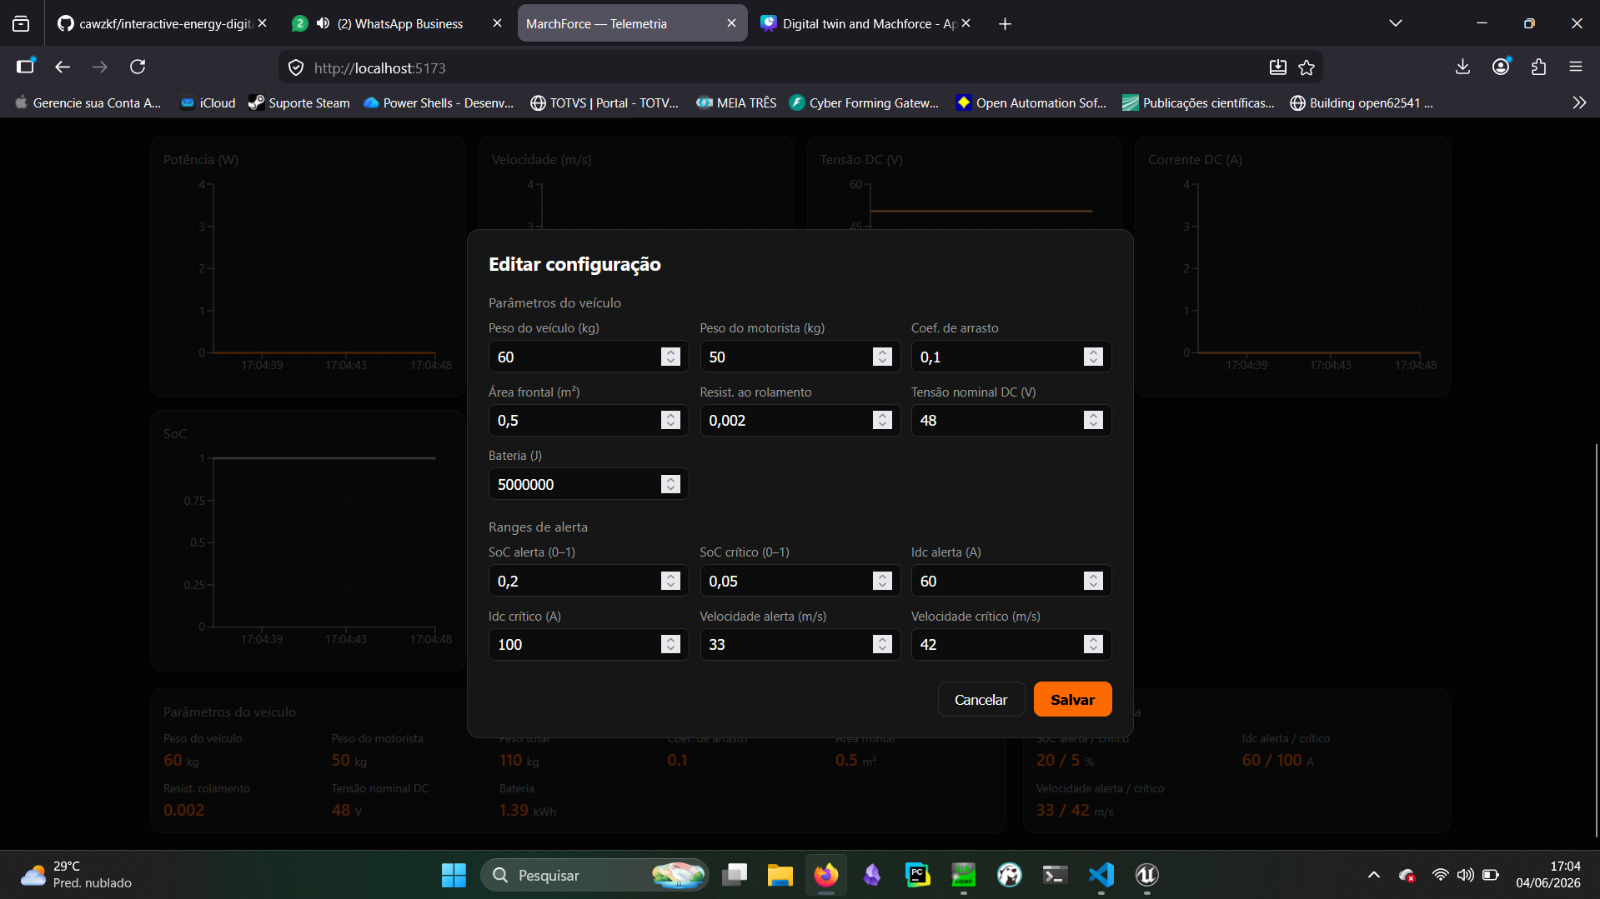
\includegraphics[width=\linewidth]{img/config_modal.jpg}
\caption{Modal de edição de configuração na dashboard: parâmetros do veículo (massas, $C_d$, área frontal, $C_r$, tensão nominal, capacidade da bateria) e limiares de alerta (SoC, corrente DC e velocidade).}
\label{fig:modal}
\end{figure}

\chapter{Metodologia}

A implementação foi realizada em Python utilizando a API oficial do simulador CARLA \cite{dosovitskiy2017carla}. O sistema é estruturado conforme a RAMI 4.0:

\begin{itemize}
\item \textbf{Integração}: aquisição de dados do CARLA (\code{src/infra/carla_client.py}, \code{src/infra/sources.py}) e publicação no MQTT (\code{src/application/acquisition_service.py})
\item \textbf{Funcional}: modelo energético e diagnóstico (\code{src/domain/}) e processamento (\code{src/application/processing_service.py})
\item \textbf{Informação}: MQTT (\code{src/infra/mqtt_client.py}), persistência (\code{src/infra/timescale_repository.py}) e AAS/BaSyx (\code{src/application/twin_service.py}, \code{twin_sync_service.py})
\item \textbf{Comunicação}: servidor OPC UA (\code{src/application/opcua_service.py}), enlace LoRa (\code{src/application/lora_service.py}) e API/WebSocket (\code{src/api/server.py})
\end{itemize}

O isolamento entre camadas é garantido por portas (interfaces abstratas em \code{src/application/ports.py}) e adaptadores concretos em \code{src/infra} e \code{src/application}.

\chapter{Arquitetura do Sistema}

\section{Visão Geral Arquitetural}

A arquitetura foi estruturada segundo o princípio de separação de responsabilidades, alinhada à RAMI 4.0. O objetivo principal é garantir desacoplamento entre o modelo energético e a infraestrutura externa (CARLA, MQTT, TimescaleDB, BaSyx, OPC UA, LoRa), mediado por um barramento de mensagens.

\section{Diagrama de Componentes}

\begin{figure}[h]
\centering
\begin{tikzpicture}[font=\sffamily,
  comp/.style={draw=mfSteel, fill=white, rounded corners=2pt, line width=0.8pt, minimum width=2.4cm, minimum height=1.15cm, align=center},
  bus/.style={draw=mfOrange, fill=mfMist, rounded corners=3pt, line width=1.1pt, minimum width=13.4cm, minimum height=0.95cm, align=center},
  dep/.style={-{Latex[length=2mm]}, mfGraphite, line width=0.7pt},
  tl/.style={font=\scriptsize\itshape, text=mfGraphite, fill=white, inner sep=1.2pt},
  st/.style={font=\scriptsize\itshape, text=mfGraphite}]
\tikzset{umlicon/.pic={\draw[mfSteel,fill=mfMist,line width=0.5pt](0,0)rectangle(0.32,0.38);\draw[mfSteel,fill=mfMist,line width=0.5pt](-0.07,0.07)rectangle(0.05,0.14);\draw[mfSteel,fill=mfMist,line width=0.5pt](-0.07,0.22)rectangle(0.05,0.29);}}
\node[comp] (acq) {{\st «component»}\\\textbf{Acquisition}\\{\scriptsize CARLA}};
\node[comp, right=3.2cm of acq] (proc) {{\st «component»}\\\textbf{Processing}};
\node[bus] (bus) at ($(acq)!0.5!(proc) + (0,-1.9)$) {{\st «message bus»}\quad\textbf{MQTT Broker}};
\node[comp, minimum width=2.2cm] (db)  at ([xshift=-5.4cm,yshift=-1.95cm]bus.south) {{\st «component»}\\\textbf{Timescale}};
\node[comp, minimum width=2.2cm] (api) at ([xshift=-2.7cm,yshift=-1.95cm]bus.south) {{\st «component»}\\\textbf{API / WS}};
\node[comp, minimum width=2.2cm] (opc) at ([xshift=0cm,yshift=-1.95cm]bus.south) {{\st «component»}\\\textbf{OPC UA}};
\node[comp, minimum width=2.2cm] (twin)at ([xshift=2.7cm,yshift=-1.95cm]bus.south) {{\st «component»}\\\textbf{TwinSync}};
\node[comp, minimum width=2.2cm] (lora)at ([xshift=5.4cm,yshift=-1.95cm]bus.south) {{\st «component»}\\\textbf{LoRa}};
\foreach \n in {acq,proc,db,api,opc,twin,lora}{\pic at ([xshift=-0.44cm,yshift=-0.48cm]\n.north east){umlicon};}
\draw[dep] (acq.south) -- (acq.south|-bus.north) node[tl,midway]{publish: raw};
\draw[dep] ([xshift=-0.45cm]proc.south|-bus.north) -- ([xshift=-0.45cm]proc.south) node[tl,midway,left=0pt]{deliver: raw};
\draw[dep] ([xshift=0.45cm]proc.south) -- ([xshift=0.45cm]proc.south|-bus.north) node[tl,midway,right=0pt]{publish: processed};
\draw[dep] (bus.south-|db.north)  -- (db.north);
\draw[dep] (bus.south-|api.north) -- (api.north);
\draw[dep] (bus.south-|opc.north) -- (opc.north) node[tl,pos=0.55]{deliver: processed};
\draw[dep] (bus.south-|twin.north)-- (twin.north);
\draw[dep] (bus.south-|lora.north)-- (lora.north);
\end{tikzpicture}
\caption{Diagrama de componentes (UML): produtores e consumidores acoplados apenas pelo barramento MQTT. \code{Acquisition} publica em \code{telemetry/raw}; \code{Processing} consome \code{raw}, executa o modelo energético e publica em \code{telemetry/processed}; os demais componentes assinam \code{processed}.}
\label{fig:componentes}
\end{figure}

\FloatBarrier

\section{Responsabilidades por Camada}

\subsection{Camada de Integração (CARLA)}
Obter velocidade ($v$), aceleração ($a$) e passo de tempo ($dt$) e publicar a leitura bruta no MQTT. Não realiza cálculos energéticos. Inclui câmera de perseguição e controle manual por teclado (WASD), com alternância para piloto automático (Traffic Manager).

\subsection{Camada Funcional -- Domínio}
Modelo físico-matemático: cálculo de forças, potência, integração discreta de energia, atualização do SoC e diagnóstico. Sem dependência direta do CARLA.

\subsection{Camada Funcional -- Aplicação}
Consome o tópico bruto, invoca \code{update(v,a,dt)}, deriva as grandezas de barramento DC ($V_{dc}$, $I_{dc}$), persiste a série temporal e republica o estado processado no MQTT.

\subsection{Camada de Informação}
Barramento MQTT, persistência por sessão em TimescaleDB e sincronização dos submodelos AAS via REST no BaSyx (alimentado pelo \code{TwinSyncService}).

\subsection{Camada de Comunicação}
Expõe as variáveis energéticas em um servidor OPC UA (\code{opc.tcp://<host>:4840/marchforce/}), entrega telemetria à dashboard por API REST + WebSocket e envia telemetria resumida ao box por LoRa.

\section{Fluxo de Execução}

O fluxo de telemetria é apresentado como diagrama de sequência UML na Figura~\ref{fig:sequencia}.

\begin{figure}[h]
\centering
\resizebox{\textwidth}{!}{%
\begin{sequencediagram}
\newthread{c}{:CARLA}
\newinst[1]{a}{:Acquisition}
\newinst[1]{b}{:MQTT Broker}
\newinst[1]{p}{:Processing}
\newinst[1]{k}{:Consumidores}
\mess{c}{tick: v, a, dt}{a}
\mess{a}{publish: telemetry/raw}{b}
\mess{b}{deliver: raw}{p}
\mess{p}{publish: telemetry/processed}{b}
\mess{b}{deliver: processed}{k}
\end{sequencediagram}}
\caption{Diagrama de sequência (UML) do fluxo de telemetria: a aquisição publica leituras brutas, o processamento executa o modelo e republica o estado processado, e os consumidores (TimescaleDB, API/WebSocket, OPC UA, BaSyx, LoRa) assinam o tópico processado.}
\label{fig:sequencia}
\end{figure}

A latência do caminho de dados foi medida em operação: da publicação no tópico \code{raw} até a entrega do \code{processed} (248 amostras), o atraso médio foi de \textbf{5,7\,ms} (mediana 4,8\,ms; p95 9,3\,ms; máx.\ 24,1\,ms), bem abaixo do passo de simulação de 100\,ms, sustentando a operação em tempo compatível com o passo discreto (RNF4). A entrega adicional à dashboard por WebSocket é local e de sobrecarga desprezível.

\section{Modos de Operação (Fonte Plugável)}

Como todo o pipeline consome exclusivamente do barramento MQTT, a fonte de telemetria é \emph{plugável}: trocá-la não altera processamento, persistência, OPC UA, AAS, LoRa ou dashboard (RNF1). São suportados três modos:

\begin{itemize}
  \item \textbf{CARLA}: a aquisição roda no host (que possui a \textit{wheel} do CARLA), lê o veículo no simulador, controlado por teclado (WASD), e publica em \code{marchforce/telemetry/raw} (\code{ACQ_SOURCE=carla}, alvo \texttt{make run-carla}).
  \item \textbf{Simulador ou sensores reais}: o simulador embutido publica telemetria sintética no mesmo tópico (\code{ACQ_SOURCE=sim}, padrão de \texttt{make run}); quando o B.O.M. for liberado, os sensores reais publicam a leitura bruta no \code{raw} pela ponte RS485$\rightarrow$MQTT, \emph{sem qualquer alteração no restante do sistema}: produtores e consumidores nunca se conhecem.
  \item \textbf{Demo}: a dashboard gera telemetria sintética no próprio navegador (\code{useDemoTelemetry}), sem \textit{backend}, MQTT ou CARLA, permitindo demonstrar a interface com o \textit{stack} desligado.
\end{itemize}

\section{Justificativa Arquitetural}

A estratificação RAMI 4.0, associada ao barramento MQTT e às portas/adaptadores, isola o modelo físico-matemático da infraestrutura de integração e comunicação, permitindo validação independente, testes unitários e substituição de fontes de dados (e.g., hardware real, ponte RS485) sem alteração da lógica do modelo.

\chapter{Resultados Esperados}

O protótipo implementado apresenta:

\begin{itemize}
\item Estimativa energética coerente, validada por 89 testes unitários e simulação sintética
\item Indicadores estratégicos calculados em tempo real
\item Barramento MQTT desacoplado e persistência temporal por sessão
\item Sincronização com AAS via Eclipse BaSyx (REST + MQTT)
\item Exposição das variáveis via OPC UA (parametrizado), cobrindo as camadas de Informação e Comunicação da RAMI 4.0
\item Dashboard web (React) com telemetria ao vivo, pista do trajeto, alertas e edição de configuração
\item Telemetria resumida ao box via enlace LoRa
\end{itemize}

\chapter{Validação do Modelo}

\section{Metodologia de Verificação}

Verificação por comparação entre o modelo implementado e o cálculo analítico direto, em cenário sintético de três fases, utilizando a configuração de referência (Tabela~\ref{tab:params}):

\begin{enumerate}
    \item \textbf{Aceleração} (0--15\,s): $a = 2{,}0$\,m/s$^2$, $v$ de 0 a 30\,m/s
    \item \textbf{Cruzeiro} (15--40\,s): $a = 0$, $v = 30$\,m/s
    \item \textbf{Frenagem regenerativa} (40--60\,s): $a = -1{,}5$\,m/s$^2$, $v$ de 30 a 0\,m/s
\end{enumerate}

Trata-se de uma \emph{verificação de consistência interna} (\textit{code verification}): o modelo é confrontado com a mesma formulação analítica que implementa, o que evidencia ausência de erros de implementação, mas \emph{não} constitui validação experimental contra dados reais. Os números desta seção usam a configuração de referência (Tabela~\ref{tab:params}, veículo de passeio); as figuras de \textit{runtime} (dashboard, OPC UA, BaSyx) usam a configuração de protótipo leve, de modo que seus valores absolutos diferem desta tabela.

\section{Resultados Quantitativos}

\begin{table}[h]
\centering
\caption{Verificação de energia acumulada por fase (configuração de referência)}
\label{tab:validation}
\begin{tabular}{@{}lrrr@{}}
\toprule
\textbf{Fase} & \textbf{$E_{modelo}$ (kJ)} & \textbf{$E_{analitico}$ (kJ)} & \textbf{Resíduo (\%)} \\
\midrule
Aceleração (0--15\,s)  & 760,22  & 760,22  & 0,0000 \\
Cruzeiro (15--40\,s)   & 447,41  & 447,41  & 0,0000 \\
Frenagem (40--60\,s)   &   0,00  &   0,00  & 0,0000 \\
\midrule
\textbf{Total}         & 1207,63 & 1207,63 & 0,0000 \\
\bottomrule
\end{tabular}
\end{table}

O resíduo nulo confirma a \emph{consistência interna} da implementação (ausência de erros numéricos frente à formulação adotada), e não uma validação experimental. A fase de frenagem aparece com energia acumulada nula porque a tabela contabiliza apenas a energia de \emph{tração} ($P>0$); a recuperação regenerativa não soma energia de tração e se manifesta na recuperação do SoC (Figura~\ref{fig:validation}, painel c: 97,3\% $\rightarrow$ 98,3\%).

\section{Análise Gráfica}

\begin{figure}[h]
\centering
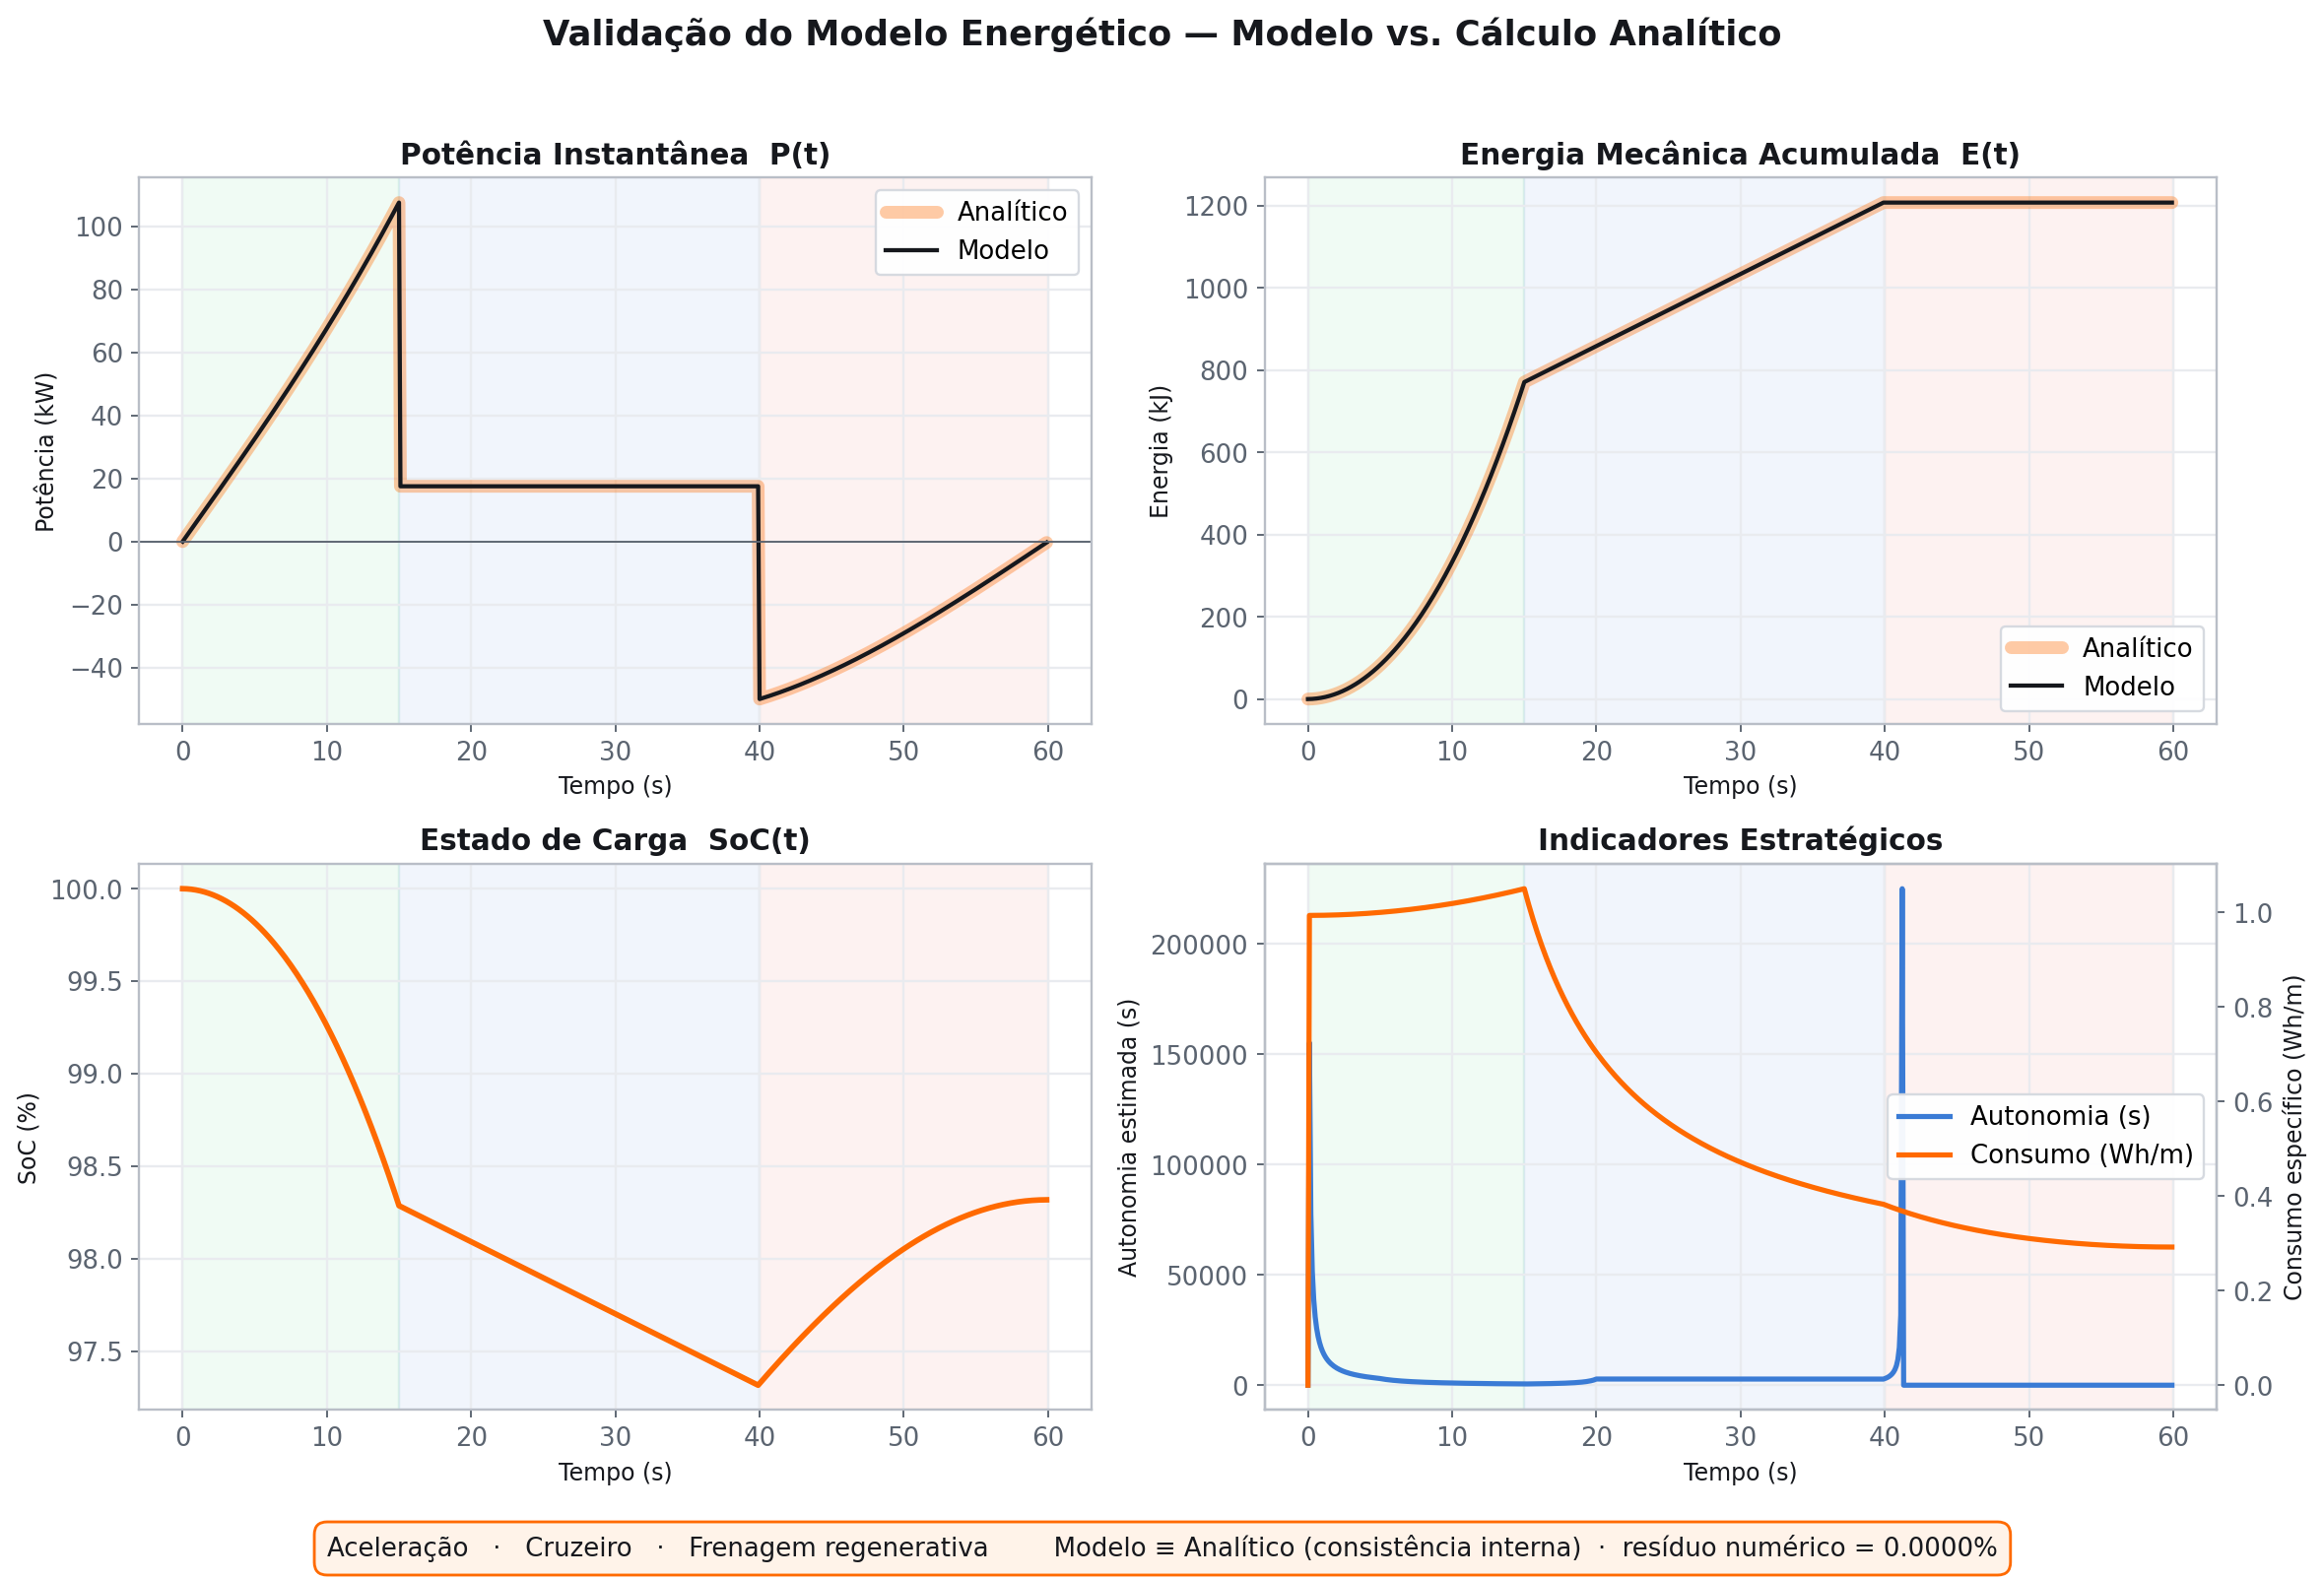
\includegraphics[width=\textwidth]{img/validation_plots.png}
\caption{Validação: (a) potência instantânea, (b) energia mecânica, (c) SoC, (d) indicadores estratégicos.}
\label{fig:validation}
\end{figure}

\FloatBarrier

\begin{itemize}
    \item \textbf{P(t)}: modelo e analítico sobrepostos; cruzeiro em $\approx$17,5\,kW; frenagem com pico de $\approx$--50\,kW
    \item \textbf{E(t)}: crescente em tração, estável em frenagem
    \item \textbf{SoC(t)}: 100\% $\rightarrow$ 97,3\% em tração; recupera para 98,3\% com regeneração
    \item \textbf{Indicadores}: autonomia $\approx$2800\,s em cruzeiro; consumo específico $\approx$0,38\,Wh/m (380\,Wh/km)
\end{itemize}

\section{Classificação da Verificação}

Esta validação caracteriza uma \textit{verificação de implementação} (\textit{code verification}). A \textit{validação experimental} contra dados reais é prevista como trabalho futuro.

\chapter{Conclusão}

O protótipo desenvolvido integra modelagem física simplificada com ambiente de simulação realista (CARLA), barramento de telemetria desacoplado (MQTT), persistência temporal (TimescaleDB), representação formal via Asset Administration Shell (Eclipse BaSyx), exposição industrial via OPC UA e visualização web em tempo real, cobrindo as camadas de Integração, Funcional, Informação e Comunicação da RAMI 4.0. Os 89 testes unitários e a verificação analítica confirmam a correção numérica do modelo, enquanto a arquitetura desacoplada por portas e adaptadores --- com configuração integral por ambiente, sem \textit{hardcoding} --- permite evolução futura para sistemas embarcados, integração com hardware real e a ponte canônica OPC UA $\rightarrow$ AAS via BaSyx DataBridge.

\printbibliography

\end{document}
